\documentclass[a4paper,11pt,notitlepage]{report}
%fleqn

\usepackage[italian]{babel}
\usepackage{amsmath, amssymb}
\usepackage{amsthm}
\usepackage{amstext}
\usepackage{array}
\usepackage{graphicx,color,psfrag,pgfplots}
\usepackage[tight]{subfigure}
\usepackage[bf,small]{caption}
\usepackage{bbm}

\usepackage{natbib}

%%%%%%%%%%%%%%PER IL BOX
\usepackage{tikz}
\usetikzlibrary{shapes,positioning,arrows,calc,shadows}
\tikzstyle{abstractbox} = [draw=black, fill=white, rectangle, 
  inner sep=11pt, style=rounded corners]%, drop shadow={fill=black,
  %opacity=1}]
  \tikzstyle{abstracttitle}=[fill=white]
  \newcommand{\mybox}[3][fill=white]{
    \begin{center}
      \begin{tikzpicture}
        \node [abstractbox, #1] (box)
        {\begin{minipage}{0.95\linewidth}
%           \setlength{\parindent}{2mm}
           \footnotesize #2
          \end{minipage}};
        \node[abstracttitle, right=11pt] at (box.north west) {#3};
      \end{tikzpicture}
    \end{center}
  }
%%%%%%%%FINE PER IL BOX


%%%%%%%%%%%%%%%%%%%%%%%%%%%%%%%%%%
\usepackage{listings}
\usepackage{color}

\definecolor{mygreen}{rgb}{0,0.6,0}
\definecolor{mygray}{rgb}{0.5,0.5,0.5}
\definecolor{mymauve}{rgb}{0.58,0,0.82}


\lstdefinestyle{customc}{
  belowcaptionskip=1\baselineskip,
  breaklines=true,
  frame=single,
  xleftmargin=\parindent,
  language=C++,
  showstringspaces=false,
  basicstyle=\footnotesize\ttfamily,
  keywordstyle=\bfseries\color{green!40!black},
  commentstyle=\itshape\color{purple!40!black},
  identifierstyle=\color{black},
  stringstyle=\color{purple},
  %morekeywords={}  
}

\lstdefinestyle{customasm}{
  belowcaptionskip=1\baselineskip,
  frame=L,
  xleftmargin=\parindent,
  language=[x86masm]Assembler,
  basicstyle=\footnotesize\ttfamily,
  commentstyle=\itshape\color{purple!40!black},
}


\lstdefinestyle{general}{ %
  backgroundcolor=\color{white},
  basicstyle=\footnotesize,       
  breakatwhitespace=false,       
  breaklines=true,                 
  captionpos=b,
  commentstyle=\color{mygreen},
  deletekeywords={...},            
  escapeinside={\%*}{*)},
  extendedchars=true,   
  frame=lines,
  %none L false leftline  topline bottomline shadowbox single lines 
  keepspaces=true,                
  keywordstyle=\color{blue},       
  language=C++,                 
  morekeywords={Real,UInt},           
  %numbers=left,
  %numbersep=5pt,              
  %numberstyle=\tiny\color{mygray}, 
  rulecolor=\color{black},
  showspaces=false,        
  showstringspaces=false,         
  showtabs=false,                  
  %stepnumber=1,                   
  stringstyle=\color{mymauve},
  tabsize=2,                      
  title=\lstname                  
}

\lstset{escapechar=@,style=customc}
%%%%%%%%%%%%%%%%%%%%%%%%%%
\usepackage{booktabs}
\usepackage{enumitem}
\usetikzlibrary{patterns}
\newcommand{\vect}[1]{\mathbf{#1}}
\newcommand{\classe}[1]{\emph{#1}}
\newcommand{\referenza}[1]{[\ref{#1}]}
\newcommand{\referenzaeq}[1]{(\ref{#1})}
\newcommand{\figref}[1]{( Fig.\ref{#1} )}
\theoremstyle{plain}
\newtheorem{teorema}{Teorema}
\graphicspath{{img/}}

\usetikzlibrary{calc,decorations.markings,positioning}

\begin{document}

\begin{titlepage}
\begin{center}
    { \scshape 
    Laurea magistrale\\
    in ingegneria matematica\\
    }
\end{center}
\vspace{1.2cm}
\begin{flushleft}
		\Large
		Progetto per il corso di \\
		Programmazione Avanzata per il Calcolo Scientifico.\\
		\vspace{1.5cm}
\end{flushleft}
\begin{figure}[h]
		\centering
		
\includegraphics[width=0.25\textwidth]{logo-polimi}
		\vspace{1cm}
\end{figure}
\begin{center}
{ \bfseries  {\Large Implementazione in LifeV dell'algoritmo di Riduzione Gerarchica di Modello}\\
\vspace{0.2cm} }
\end{center}
\vspace{0.4cm}
\begin{flushright}
		\Large
		Progetto svolto da:\\
		Matteo Carlo Maria Aletti\\
		Matr. 783045\\
		Andrea Bortolossi\\
		Matr. 783023\\
		\vspace{1.5cm}
\end{flushright}
\begin{center}
Anno Accademico 2012--2013
\end{center}

\end{titlepage}
\clearpage
\tableofcontents
\chapter{Introduzione}

In molti problemi di interesse ingegneristico i fenomeni in esame presentano
direzioni preferenziali. Ad esempio in emodinamica \`e possibile incontrare problemi
simili dove la direzione del flusso \`e dominante rispetto alla dinamica
in direzione trasversale.
L'obbiettivo del progetto \`e l'implementazione in \texttt{LifeV} di un 
risolutore per un problema di diffusione trasporto reazione ( Advection Diffusion 
Reaction - ADR) 3D, basato sulla tecnica di Riduzione Gerarchica di Modello
(Hierarchical Model Reducation - HiMod).

HiMod si propone di sfruttare l'informazione
sulla presenza di una direzione dominante per ridurre il costo computazionale
della risoluzione convertendo un problema tridimensionale
in diversi problemi monodimensionali accoppiati.
La riduzione \`e resa possibile da uno sviluppo in serie di 
Fourier generalizzate della soluzione solo nella direzione trasversale. 
L'idea \`e quindi di approssimare soltanto i primi coefficienti di Fourier della soluzione.

\`E chiaro che il metodo non potr\`a essere competitivo rispetto al
metodo degli elementi finiti nel caso di problemi senza dinamiche dominanti,
tuttavia, dove la dinamica trasversale \`e semplice, consente di ottenere
una buona approssimazione del fenomeno, superiore rispetto a un modello
ridotto monodimensionale, ma senza i costi di una risoluzione 3D.

Approfondimenti riguardo alla Riduzione Gerarchica di Modello si possono trovare in
\cite{perotto:2008},\cite{perotto:2009},\cite{perotto:2012} e in \cite{zilio:himod} dove il metodo \`e stato 
applicato in un contesto bidimensionale (con condizioni di Dirichlet al bordo laterale) e parzialmente sviluppato dal punto di vista
teorico nel caso tridimensionale.

Nel progetto ci siamo focalizzati sull'implementazione del metodo in un contesto 
tridimensionale con una geometria semplice, ma con diverse tipologie di condizioni al bordo.
In particolare abbiamo implementato le basi istruite: una particolare scelta della base di Fourier
per la direzione trasversale in grade di incorporare le condizioni al bordo.


\section{Descrizione del metodo}

In questa sezione presenteremo le basi teoriche del metodo, applicandolo a un problema
di diffusione trasporto e reazione.

Consideriamo il seguente problema in un generico dominio $\Omega$, visto che il metodo 
\`e stato pensato soprattutto per applicazioni in emodinamica, consideriamo un dominio 
di forma tubolare
\begin{equation}
\label{eq: problema forte}
\begin{cases}
-\mu\Delta u + \vect{b}\cdot \nabla u + \sigma u = f & \text{in $\Omega$}\\
u=u_{in} & \text{su $\Gamma_{in}$}\\
\frac{\partial u}{\partial \vect{n}}=0 & \text{su $\Gamma_{out}$ }\\
u=0 & \text{su $\Gamma _{vaso}$} \\
\end{cases}
\end{equation}
\begin{center}
\begin{tikzpicture}
[scale=0.8]
\def\xi{0};
\def\xo{7};
\def\c{3.5};
\def\r{1};
\def\sig{2};
\def\rmax{0.5};
\def\rtot{\rmax+\r};

\draw[thick] (\xi,0) arc (90:270:0.3cm and \r cm);
\draw[dashed,thick] (\xi,-2*\r) arc (-90:90:0.3cm and \r cm);

\draw[thick] (\xo,0) arc (90:270:0.3cm and \r cm);
\draw[thick] (\xo,-2*\r) arc (-90:90:0.3cm and \r cm);

% \draw[->] (-2,0) -- (2,0);
% \draw[->] (0,-2) -- (0,2);
\draw[thick,parametric,domain=-\xi:\xo,samples=200,variable=\t] plot ({\t},{\rmax*exp{-pow(\t-\c,2)/\sig}});
\draw[thick,parametric,domain=-\xi:\xo,samples=200,variable=\t] plot ({\t},{-2*\r-\rmax*exp{-pow(\t-\c,2)/\sig}});
\draw[thick,parametric,domain=-\xi:\xo,samples=200,variable=\t,dashed] plot ({\t},{-\r});
\def\po{0.9};
\node[below] at (\xo*\po,-\r) {$\Omega_{1D}$};
\draw[pattern=north west lines, pattern color=gray, thick] (\c,-\r) ellipse (0.3 and \rtot);
\node[below] at (\c,-2*\r-\rmax) {$\gamma_x$};
\node[left] at(\xi-0.2,-\r) {$\Gamma_{in}$};
\node[right] at(\xo +0.2,-\r) {$\Gamma_{out}$};
\node at (\xi +0.5,-\r-0.7) {$\Omega$};
\node at (\c +2,-2*\r-0.4) {$\Gamma_{vaso}$};
\end{tikzpicture}
\end{center}
dove i coefficienti che compaiono nell'equazione sono tali per cui il problema variazionale associato 
sia ben posto in $V=H^1_{\Gamma_{IN}\cup\Gamma_{vaso}}(\Omega)$.
Immaginiamo di suddividere il dominio $\Omega$ in slice poste trasversalmente alla direzione longitudinale 
\begin{equation}
\label{eq:volume ridotto}
\Omega=\bigcup_{x\in \Omega_{1D}}\gamma_x.
\end{equation}
Ogni slice viene indicata con $\gamma_x$.
Lungo $\gamma_x$ vengono utilizzate funzioni spaziali differenti rispetto
a quelle utilizzate lungo $\Omega_{1D}$. 
Nel caso del tubo a sezione rettangolare, sul quale il codice si focalizzer\`a, $\Omega$ si riduce a $(0,L_x)\times\gamma$ 
dove $\gamma_x=\gamma=(0,L_y)\times(0,L_z)\quad\forall x\in(0,L_x)$
\begin{center}
\begin{tikzpicture}
[scale=1.5]

\draw [thick] (2,0) rectangle (3,1);
\node at (-0.25,1.25) {$\Gamma_{in}$};
\node at (3.3,0.5) {$\Gamma_{out}$};
\node at (2,1.75) {$\Gamma_{vaso}$};
\node at (0.5,0.4) {$\gamma$};
% \node at (0.7,0.88) {$\gamma}$};
\node at (3.5,-0.2) {$\Omega_{1D}$};


\draw [thick] (2,1)--(0,2)--(1,2)--(3,1);
\draw [thick] (2,0)--(0,1)--(0,2);

\draw [dashed,thick] (0,1)--(1,1)--(1,2);
\draw [dashed,thick] (1,1)--(3,0);

\draw [pattern=north west lines, pattern color=gray, thick] (0.5,0.75) rectangle (1.5,1.75);

\draw [thick,dashed, ->] (-0.5,2)--(3.5,0);

\end{tikzpicture}
\end{center}

Per gestire un dominio di forma generica \`e necessario utilizzare una mappa con la quale ricondursi ad un 
dominio di riferimento (si veda \cite{perotto:2008}. La teoria delle basi istruite, tuttavia, non \`e, ora, in grado di coprire 
il caso della mappa\footnote{In fase di implementazione abbiamo cominciato ad inserire le funzionalit\`a relative alla
mappa, ma ci siamo limitati ad aprire un branch sul repository (\texttt{20130710\_HiModMap})	 che, pur essendo praticamente 
completato, abbiamo dovuto abbandonare essendo incompatibile con le basi istruite. 
Con un altro tipo di base, ad esempio i polinomi di Legendre, \`e possibile recuperare il branch e 
completare l'implementazione.}.

Introduciamo alcuni spazi funzionali utili per ambientare correttamente il metodo.
Su $\Omega_{1D}$ utilizziamo lo spazio $V_{1D}=H^1_{\Gamma_{in}}(\Omega_{1D})$, 
mentre sulla fibra trasversale $\gamma$ introduciamo le basi modali $\left\{ \varphi_k \right\}_{k=1}^\infty$ 
ortonormali rispetto al prodotto scalare di $L^2(\gamma)$.
Quest'ultime definiscono su $\gamma$ lo spazio funzionale $V_{\gamma}:=span\left(\{\varphi_k\}_{k=1}^\infty\right)$.
\`E possibile dimostrare che, chiuso rispetto ad una opportuna norma, lo spazio $V_{1D}\otimes V_{\gamma}$ \`e isometricamente 
isomorfo a $V$. Per ulteriori dettagli sulla teoria e sulla notazione si pu\`o vedere la tesi di laurea di A. Zilio \cite{zilio:himod}.

Definiamo ora il sottospazio generato solo dai primi m modi ovvero  $V^m_{\gamma_x}:=span\{\varphi_1,...,\varphi_m\}$ e combiniamolo con $V_{1D}$, il risultato di tale operazione \`e il seguente spazio ridotto:
\begin{equation}
\label{spazio: ridotto}
V_m:=\left\{v_m(x,y,z)=\sum^m_{k=1}\varphi_k(y,z)\tilde{v}_k(x) ,\:\:con\:\:\tilde{v}_k\in V_{1D}\right\}.
\end{equation}

Questo \`e l'ambiente funzionale in cui opera HiMod.
L'ortogonalit\`a in $L^2(\gamma)$ implica che i coefficienti  $\tilde{v}_k$ che compaiono nella \eqref{spazio: ridotto} 
siano il risultato del seguente prodotto scalare
\begin{displaymath}
\tilde{v}_k(x)=\int_{\gamma}\varphi_k(y,z)v_m(x,y,z)\,dydz\quad\forall k=1\ldots m
\end{displaymath}
osserviamo come questi rappresentino, puntualmente, i coefficienti di Fourier della soluzione esatta rispetto alla base 
utilizzata sulla fibra trasversale.

La convergenza di una soluzione $u_m$ tale che soddisfi il problema \eqref{eq: problema forte}, nella sua forma variazionale
posta sul sottospazio $V_m$, discende dalle seguenti propriet\`a:
\begin{itemize}
\item[-] $V_m \subset V$ $\forall m\in \mathbb{N}$, ossia che lo spazio ridotto $V_m$ \`e \textbf{conforme} in $V$;
\item[-] $\displaystyle \lim_{m\to +\infty} \left(\inf_{v_m\in V_m}\mid\mid v-v_m\mid\mid\right)=0$ 
per ogni $v \in V$, ossia che vale la \textbf{propriet\`a di approssimazione} di $V_m$ rispetto a $V$;
\end{itemize}
Quest'approccio pu\`o essere esteso al caso di condizioni sulla parete laterale diverse dalle condizioni di Dirichlet omogenee.
In questo progetto abbiamo implementato l'approccio delle basi istruite, ma altre scelte sono possibili.

\section{Forma matriciale}
Per ogni $m\in\mathbb{N}$ consideriamo il seguente problema ridotto 

\noindent\emph{Trovare $u_m\in H^1(\Omega_{1D})\otimes V_{\gamma}^m$ tale che $\left.u_m\right|_{\Gamma_{in}}$ sia uguale alla proiezione del dato di Dirichlet 
su $V_\gamma^m$ e valga}
\begin{multline*}
\int_\Omega\left(\mu\nabla u_m\nabla v_m + \vect{b}\cdot\nabla u_mv_m+\sigma u_mv_m\right)\,d\Omega\quad \forall v_m\in V_m
=\int_\Omega fv \,d\Omega
\end{multline*}

Utilizziamo l'espansione di $u_m(x,y,z)$ 
rispetto alla base di Fourier 
\begin{equation}
\label{eq: espansione himod}
u_m(x,y,z)=\sum_{j=k}^m\tilde{u}_j(x)\varphi _j(y,z),\quad\tilde{u}_j(x)=\int_{\gamma}u_m(x,y,z) \varphi_j(y,z)\,dydz
\end{equation}
consideriamo inoltre funzioni test della forma 
$$v_m=\vartheta(x)\varphi _k(y,z),\quad \vartheta(x)\in V_{1D}\text{ e }
k=1,...m.$$ Il problema assume la seguente forma:

\begin{equation*}
\begin{split}
&\sum_{j=1}^m 
\int_\Omega\mu\nabla (\tilde{u}_j(x)\varphi _j(y,z))\nabla (\vartheta(x)\varphi _k(y,z))\,dxdydz\\
&+\int_\Omega(\vect{b}\nabla (\tilde{u}_j(x)\varphi _j(y,z))+\sigma\tilde{u}_j(x))\vartheta(x)\varphi _k(y,z)\,dxdydz\\
&=\int_\Omega f\vartheta(x)\varphi _k(y,z)\,dxdydz\\
\end{split}
\end{equation*}

Svolgendo l'operatore gradiente si ottiene:

\begin{equation*}
\begin{split}
&\sum_{j=1}^m
\int_\Omega\mu( \partial_x\tilde{u}_j \partial_x\vartheta\varphi _j\varphi _k + \tilde{u}_j \vartheta \partial_y\varphi _j\partial_y\varphi _k + \tilde{u}_j \vartheta \partial_z\varphi _j\partial_z\varphi _k)\,dxdydz \\
&+ \int_\Omega (b_1\partial_x\tilde{u}_j\varphi _j+b_2\tilde{u}_j\partial_y\varphi _j + b_3\tilde{u}_j\partial_z\varphi_j)\vartheta\varphi _k\,dxdydz\\ 
&+ \int_\Omega \sigma\tilde{u}_j\vartheta\varphi _j\varphi _k\,dxdydz \\
&=\int_\Omega f\vartheta\varphi _k\,dxdydz
\end{split}
\end{equation*}

Vediamo come il problema 2D si sia trasformato nella ricerca di $m$ funzioni monodimensionali.
Per semplicit\`a consideriamo una partizione $\tau_h$ uniforme lungo 
la fibra di supporto 1D.
Sia $N$ il numero di vertici lungo $\Omega_{1D}$.
Il passo della partizione \`e dunque $h=\vert \Omega_{1D}\vert / (N-1)$. 

Introduciamo lo spazio agli elementi finiti lungo $\Omega_{1D}$
\begin{equation*}
\label{eq: spazio polinomiale}
X_h^r= \left\{\psi_h \in C^0(\Omega_{1D}): \psi_h \vert_K  \in \mathbb{P}_r,\forall K\in T_h \right\}.
\end{equation*}
Per semplicit\`a supponiamo di utilizzare elementi finiti di grado uno, ma
la trattazione teorica \`e del tutto equivalente nel caso si volessero usare 
polinomi di grado pi\`u alto.
Una volta introdotta la discretizzazione lungo la direzione dominante 
del fenomeno \`e possibile esprimere i coefficienti di Fuorier 
nel seguente modo
\begin{equation*}
\label{eq: coeff fourier espansi}
\tilde{u}_j(x)=\sum_{s=1}^Nu_{js}\psi_s(x).
\end{equation*}
Abbiamo quindi discretizzato completamente il problema. Tramite l'espansione modale
siamo stati in grado di ridurre il problema da 3D a $m$ problemi 1D accoppiati che ora
abbiamo discretizzato con il metodo degli elementi finiti.

Otteniamo dunque la formulazione matriciale del problema\\
\emph{Trovare $\vect{u} \in \mathbb{R}^{N\cdot m}$ tale che}
\begin{equation*}
\begin{split}
&\sum_{j=1}^m \sum_{s=1}^N
u_{js} \Bigg[ \int_\Omega\mu( \partial_x\psi_s \partial_x\psi_l\varphi _j\varphi _k + \psi_s \psi_l \partial_y\varphi _j\partial_y\varphi _k + \psi_s \psi_l \partial_z\varphi _j\partial_z\varphi _k)\,dxdydz \\
&+ \int_\Omega (b_1\partial_x\psi_s\varphi _j+b_2\psi_s\partial_y\varphi _j + b_3\psi_s\partial_z\varphi_j)\psi_l\varphi _k\,dxdydz\\ 
&+\int_\Omega \sigma\psi_s\psi_l\varphi _j\varphi _k\,dxdydz \Bigg]\\
&=\int_\Omega f\psi_l\varphi _k\,dxdydz\quad \forall \psi_l\quad l=1\ldots N\quad\forall \varphi_k\quad k=1\ldots m
\end{split}
\end{equation*}
Per chiarezza abbiamo utilizzato un doppio indice $"js"$. Esso scorre in realt\`a  un vettore,
ma \`e possibile usare un solo indice che si lega a $"js"$ nel seguente modo
$$\vect{u}_{js}=\vect{u}[i]=\vect{u}[(j-1)N+s].$$ 
Integrando prima lungo la fibra trasversale si ottiene:
\begin{equation*}
\begin{split}
TODO
\end{split}
\end{equation*}
 La matrice generata ha dimensioni $(mN)^2$, tuttavia fissata
 la frequenza della soluziona e della funzione test, ossia fissando l'indice che scorre la base modale,
 \`e possibile identificare un blocco che corrisponde ad un problema monodimensionale.
Se utilizziamo gli elementi finiti di grado uno, il blocco \`e tridiagonale e
 la matrice ha un numero di elementi non zero pari a $m^2(3N-2)$. 
 Il pattern di sparsit\`a per un caso con m=3 e N=14 \`e riportato in figura \ref{fig:pattern}.
 \begin{figure}[!h]
    \centering
    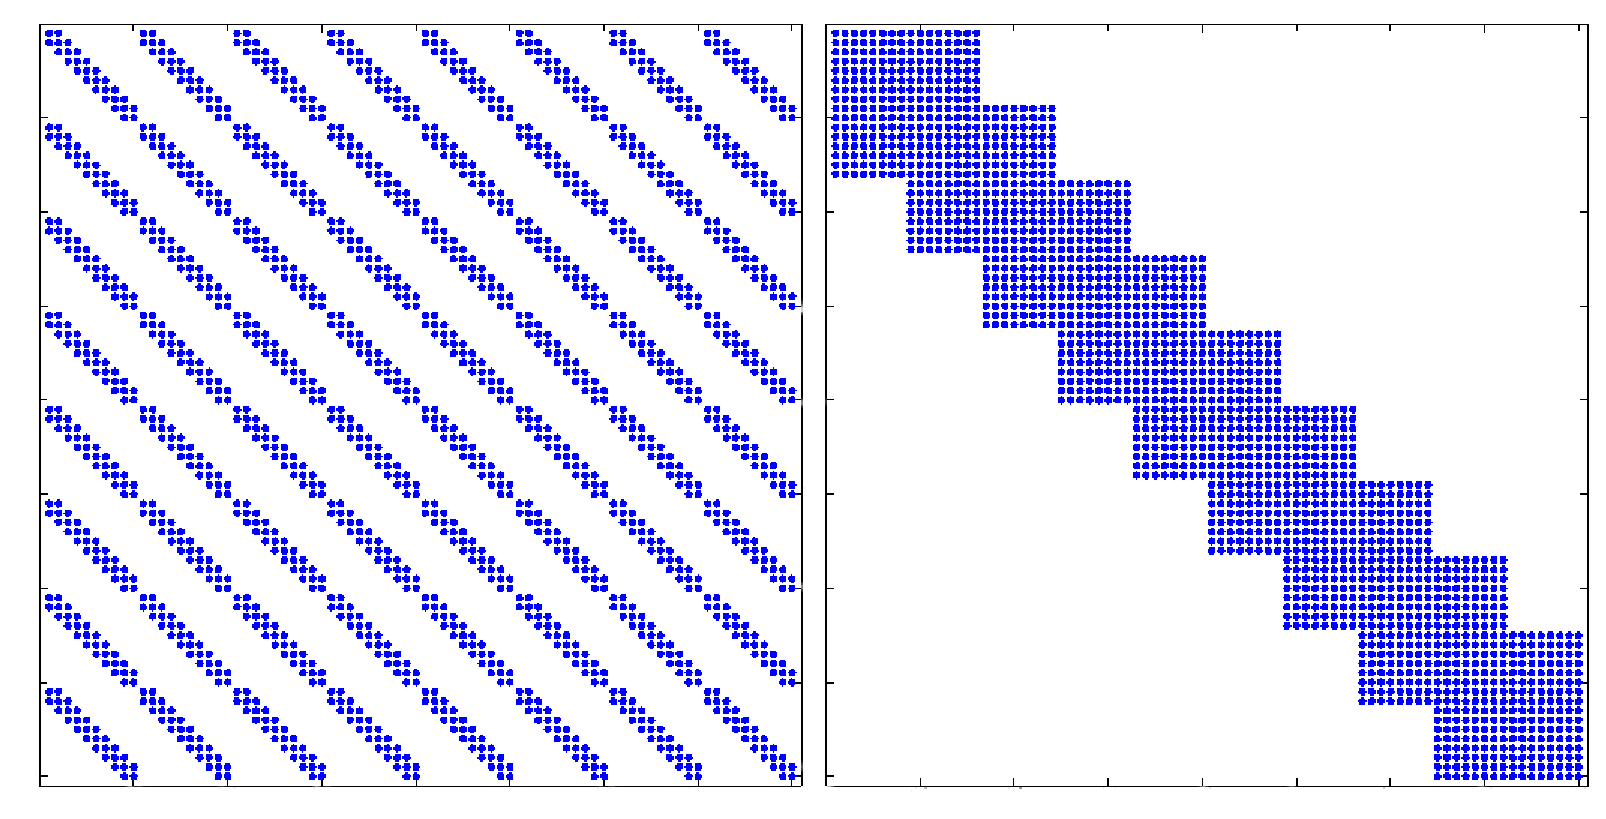
\includegraphics[scale = 0.45]{Varie/spy}
    \caption{Pattern di sparsit\`a per un caso con 9 elementi P1 e 8 modi.\\A sinistra il pattern che \`e stato poi utilizzato, a destra l'alternativa.}
    \label{fig:pattern}
\end{figure}
La matrice dei coefficienti \`e sparsa con un pattern noto a priori, ci\`o ha permesso 
 un assemblaggio pi\`u veloce in fase implementativa.
 \`E anche possibile riordinare la matrice in modo differente. Utilizzando una struttura 
 a blocchi associata ai gradi di libert\`a degli elementi finiti e non alla base modale.
 In questo modo avremmo una matrice tridiagonale a blocchi e ogni blocco sarebbe una matrice
 $m\times m$ piena. Con questa riordinamento della matrice la struttura \`e dunque quella 
 di un problema 1D dove invece che un solo grado di libert\`a associato al nodo ne sono associati $m$.
 Abbiamo implementato la prima scelta, che \`e quella suggerita in
 \cite{perotto:2008}, anche per poter sfruttare le procedure di assemblaggio 
 per gli elementi finiti 1D gi\`a presenti in LifeV.
\clearpage

\section{Basi istruite}
\label{sec: educated basis}
Le basi istruite sono state chiamate in questo modo perch\`e sono basi in grado di leggere la natura 
delle condizioni al bordo e di incorporarla all'interno della base stessa. Esse
conoscono parte del problema in esame.
Utilizzare le basi istruite equivale a imporre in maniera essenziale anche le condizioni al bordo 
naturali, come quelle di tipo Robin.
Il metodo delle basi istruite si basa sulla risoluzione di un problema agli autovalori 
ausiliario posto sulla fibra trasversale $\gamma$.\footnote{Nell'implementazione abbiamo risolto il
problema riportandolo sul quadrato di riferimento $(0,1)\times(0,1)$.} 
Introduciamo con un esempio l'algoritmo di costruzione delle basi istruite
\begin{itemize}
\item[\textbf{1.}] \textbf{Costruzione di un problema ausiliario} che rispecchi 
la natura delle condizioni alle pareti del problema originale (devono essere omogenee) e passaggio ai relativi problemi agli autovalori.
\mybox{
Nel caso si abbiano condizioni di Robin sull'intera parete del vaso, dovremo considerare il seguente problema ausiliario
\begin{equation}
\label{eq: problema RRRR}
\begin{cases}
-\Delta u(y,z)= 0 & \text{in $\gamma$}\\
\mu \nabla u(y,z) \cdot \vect{n} +\chi u(y,z)=0 & \text{su $\partial\gamma$}. \\
\end{cases}
\end{equation}
Si passi ora al problema agli autovalori associato al precedente sistema e 
ipotizzando la separazione di variabili $u(y,z)=\varphi(y)\vartheta(z)$, 
si arriva facilmente ai seguenti sottoproblemi agli autovalori
\begin{equation}
\label{eq: problema RR1}
\begin{cases}
-\varphi(y)'' = K_y\varphi(y) & \\
\mu \varphi(y)' +\chi \varphi(y) = 0 & \text{per $y=L_y$} \\
-\mu \varphi(y)'+\chi \varphi(y)=0 & \text{per $y=0$}. \\
\end{cases}
\end{equation}
\begin{equation}
\label{eq: problema RR2}
\begin{cases}
-\vartheta(z)'' = K_z\vartheta(z) & \\
\mu \vartheta(z)' +\chi \vartheta(z) = 0 & \text{per $z=L_z$} \\
-\mu \vartheta(z)'+\chi \vartheta(z)=0 & \text{per $z=0$} \\
\end{cases}
\end{equation}
}{Esempio - Robin BC}

\item[\textbf{2.}] \textbf{Identificazione del tipo di soluzione} dei problemi agli autovalori associati.

\mybox{
La generica soluzione dei sottoproblemi ottenuti \`e
\begin{equation}
\label{eq: 1sottoproblema}
\begin{array}{c}
\varphi (y)=A_ysin(\sqrt{K_y}y)+B_ycos(\sqrt{K_y}y) \\ \\
\vartheta (z)=A_zsin(\sqrt{K_z}z)+B_zcos(\sqrt{K_z}z).
\end{array}
\end{equation}

}{Esempio - Robin BC}

\item[\textbf{3.}] \textbf{Ricerca degli autovalori di un sottoproblema} tramite risoluzione dell'equazione non lineare associata ad esso, ottenuta risolvendo le condizioni di bordo.
\mybox{
Nel caso trattato in esempio le equazioni che si ottengono sono le seguenti ($x = \sqrt{K_y}$ e $w= \sqrt{K_z}$)
\begin{equation}
\label{eq: funzione autovalori}
\begin{array}{c}
f(x)= 2\mu x + tan(L_y x)\left(\chi - \frac{\mu ^2 x^2 }{\chi} \right) \\ \\
f(w)= 2\mu w + tan(L_z w)\left(\chi - \frac{\mu ^2 w^2 }{\chi} \right).
\end{array}
\end{equation}
}{Esempio - Robin BC}
\end{itemize}
Per giustificare l'algoritmo dal punto di vista teorico riportiamo solamente un teorema
che analizza un generico problema agli autovalori. Per adattarlo al nostro caso
\`e sufficiente scegliere $H=L^2(\gamma)$ e $V=H^1_{\partial\gamma_o}(\gamma)$, dove $\partial\gamma_0$ \`e il sottoinsieme
di $\partial\gamma$ dove sono imposte le condizioni di Dirichlet e la forma bilineare $a$ si riferisce alla forma variazionale
associata al problema ausiliario agli autovalori, per ulteriori dettagli si veda \cite{salsa2004equazioni}.
\begin{teorema}
\label{teo: salsa}
Siano V,H spazi di Hilbert, con H separabile, V denso in H, e tali che
l'immersione di V in H sia compatta. Sia a( , ) una forma bilineare in V,
continua, simmetrica e debolmente coerciva. 
Allora
\begin{description}
\item[(a)] $\sigma(a)=\sigma_p(a)\subset(-\lambda_0,+\infty)$. Inoltre, se la successione degli autovalori $\{\lambda_m \}_{m\geq 1}$ \`e infinita allora $\lambda_m\rightarrow +\infty$;
\item[(b)] se u ,v sono autovettori corrispondenti ad autovalori differenti, allora a(u,v) = 0 = (u,v). Inoltre, H ha una base ortonormale $\{ u_m \}_{m\geq 1}$ di autovettori di a;
\item[(c)] la successione $\{u_m / \sqrt{\lambda_0+\lambda_m} \}_{m\geq 1}$ costituisce una base ortonormale in V, rispetto al prodotto scalare
\begin{displaymath}
((u,v))=a(u,v)+\lambda_0 (u,v).
\end{displaymath}
\end{description}
\end{teorema}
$\sigma$ \`e lo spettro della forma bilineare $a$, $\sigma_p$ il suo spettro puntuale, $\lambda_0$ \`e l'eventuale costante necessaria per la debole coercivit\`a.
La base che si ottiene \`e dunque ortonormale rispetto al prodotto scalare $L^2(\gamma)$.

\mybox{
Nel caso di condizioni al bordo di Dirichlet il problema si semplifica. 
Infatti non occorre risolvere l'equazione non-lineare:	
gli autovalori che si ottengono sono noti a priori e sono della forma
\begin{equation}
\label{eq: problema agli autovalori dirichlet}
\begin{array}{c l}
K_{y,p} = \left( \frac{\pi p}{L_y}\right)^2 & p = 1, ... ,m_y\\
K_{z,q} = \left( \frac{\pi q}{L_z}\right)^2 & q = 1, ... ,m_z\\
\lambda_{p,q}=K_{y,p}+K_{z,q}.&\\
\end{array}
\end{equation}
}{Osservazione -- Caso condizioni al bordo di Dirichlet}
Numericamente, o analiticamente come nel caso di condizioni al bordo di Dirichlet, \`e possibile
trovare gli autovalori dei sottoproblemi monodimensionali. La difficolt\`a
st\`a nel legarli in modo opportuno agli autovalori del problema bidimensionale in modo che 
venga preservato l'ordinamento crescente degli autovalori 2D rispetto all'indice $k$ della base modale.
In particolare \`e necessario costruire una mappa che leghi ad ogni frequenza $k$ 
la corretta coppia $(p,q)$, per farlo abbiamo sviluppato un algoritmo che verr\`a descritto 
nel capitolo relativo all'implementazione.
\clearpage
\clearpage
\chapter{Implementazione}

L'implementazione \`e stata sviluppata all'interno dell'ambiente \texttt{LifeV}, per la compilazione abbiamo utilizzato \texttt{cmake} 
e, per la gestione del codice, abbiamo utilizzato \texttt{git}. Il codice si trova nel branch \texttt{20130507\_HiMod}.
Per la gestione di vettori e matrici e per la risoluzione del sistema lineare sono state utilizzate le strutture disponibili
in \texttt{LifeV} che sono basate su \texttt{Trilinos}, tuttavia non abbiamo approfondito la gestione 
delle strutture dati e del sistema lineare, che andrebbero sviluppate ad hoc per il metodo in esame: 
la particolare struttura a blocchi della matrice di sistema non \`e simile a nessuna delle tipiche
matrici degli elementi finiti. Per quanto riguarda la parte di assemblaggio dei sottoproblemi monodimensionali
abbiamo invece utilizzato il pacchetto di \texttt{LifeV} che sfrutta gli Expression Templates (\text{ETA}).
Il codice \`e stato sviluppato in seriale perch\`e la sua implementazione in parallelo necessita di una
struttura dati appropriata.

Prima di procedere con la descrizione dell'implementazione riportiamo le ipotesi 
di lavoro che sono state fatte per lo sviluppo del codice. Alcune si possono rilassare facilmente,
altre invece necessitano un cambiamento pi\`u sostanziale.
\begin{enumerate}[label=\Roman{*} -, ref=(\Roman{*})]
\item Il dominio di calcolo \`e un parallelepipedo $(0,L_x)\times(0,L_y)\times(0,L_y)$.
\item Griglia 1D strutturata.
\item Si considera un problema ADR stazionario con condizioni di inflow di tipo Dirichlet e di outflow di tipo Neumann omogeneo.
\item I coefficienti del problema costanti.
\item Forzante e dato di Dirichlet in ingresso sono generici.
\item Condizioni sulle pareti omogenee.
\item \`E possibile separare il problema lungo le direzioni trasversali, in due sotto problemi agli autovalori.
\end{enumerate}

Come accennato nell'introduzione teorica, la forma del dominio considerato ci consente di utilizzare con semplicit\`a le basi istruite. 
Nel caso di sezione di forma generica, la gestione di condizioni al bordo sulla parete laterale risulterebbe pi\`u complicata.
Come sviluppo successivo si potrebbe pensare di utilizzare i polinomi di Legendre al posto delle funzioni trigonometriche.
Anche nel caso di generalizzazione dei coefficienti della forma, viene presentata una possibile soluzione, 
tuttavia il codice \`e strutturato per l'utilizzo di coefficienti costanti.
L'ipotesi sulla griglia 1D strutturata riguarda soltanto alcune funzionalit\`a del post-processing.
Per quanto riguarda, invece, l'ipotesi sulle condizioni omogenee a parete, sarebbe necessario costruire un rilevamento dei dati al bordo.

In questo progetto abbiamo considerato un dominio che \`e un prodotto di intervalli, abbiamo riflettuto sulla possibilit\`a di rendere il 
codice sufficientemente generale, per poterlo estendere al caso a sezione cilindrica, ma pur essendoci delle somiglianze 
non ci \`e sembrato utile costruire una classe astratta da cui ereditare le implementazioni delle due diverse geometrie 
in quanto era possibile conservare solo l'implementazione di pochissimi metodi.

Per quanto riguarda le condizioni ai bordi di ingresso e uscita il codice permette di applicare 
condizioni di inflow di tipo Dirichlet non omogenee, le condizione di Neumann all'outflow 
disponibili sono invece  omogenee, ma l'eventuale estensione al caso non omogeneo o ad altri tipi di condizioni 
al bordo \`e molto semplice e naturale.

Dall'introduzione teorica si vede come, nella discretizzazione del problema, si fondano due parti molto diverse, 
da una lato gli Elementi Finiti, lungo la fibra di supporto, dall'altra la base modale 2D, che ricorda molto i metodi spettrali. 
L'organizzazione delle classi segue questa idea. Per prima cosa \`e stato necessario costruire delle classi in grado di risolvere
i problemi agli autovalori monodimensionali: \classe{Basis1DAbstract} fornisce un interfaccia astratta
dalla quale ereditano diverse classi che sono in grado di calcolare gli autovalori e di valutare le funzioni di base.
In secondo luogo, la classe \classe{ModalSpace} gestisce il problema agli autovalori bidemensionale,
\`e in grado di ordinare gli autovalori e costruire la mappa tra $k$ e $(p,q)$, fornisce diverse utilit\`a
per calcolare coefficienti di Fourier e altro. Essa \`e la classe che mette in relazione le due basi monodimensionali. 
Infine il collegamento tra la discretizzazione lungo la fibra di supporto e quella lungo la sezione trasversale
\`e gestito da \classe{HiModAssembler} che rappresenta l'interfaccia esterna che assembla la matrice e il termine 
noto oltre a contenere alcune utilit\`a ad esempio per il calcolo dell'errore.
Altre classi sono state sviluppate per diversi tipi di utilit\`a.

\section{Basis1dAbstract}
\classe{Basis1DAbstract} \`e la classe astratta che definisce l'interfaccia di un generico generatore di basi monodimensionali.
Le classi figlie sono degli oggetti pensati per essere utilizzati da \classe{ModalSpace}, essa infatti contiene due puntatori, 
\texttt{M\_genbasisY} e \texttt{M\_genbasisZ}, ognuno dei quali punta a una classe figlia di \classe{Basis1DAbstract}.
Le diverse classi figlie di \classe{Basis1DAbstract} si differenziano principalmente per il diverso problema agli autovalori che risolvono.
Per ora sono implementate quattro delle nove possibili combinazioni di condizioni al bordo: \classe{EducatedBasis\{DD,RR,DR,NN\}} 
ognuna di queste risolve un problema con condizioni al bordo di tipo D=Dirichlet, R=Robin e N=Neumann, il carattere di sinistra 
si riferisce al bordo sinistro dell'intervallo (0,1) il carattere di destra al bordo destro. \`E anche presente una 
classe \classe{FakeBasis}, che implementa, con un piccolo trucco, una base finta che, assegnata come base per la direzione
$z$ ( o $y$ ) ci consente di utilizzare il software come solutore bidimensionale, \`e stata sviluppata in fase di debug 
per testare separatamente i diversi tipi di basi istruite.
I problemi agli autovalori sono stati risolti nell'intervallo di riferimento $(0,1)$ e rimappati nell'intervallo fisico.
 
\subsubsection{I metodi}
Ogni classe figlia eredita pubblicamente da \texttt{Basis1DAbstract}
\begin{lstlisting}[style = general]
class Basis1DAbstract
{public:
    Basis1DAbstract();
    virtual ~Basis1DAbstract();
    void setL (const Real& L);
    
    virtual void setMu (Real const& mu );
    virtual void setChi(Real const& chi);
    
    virtual Real chi() const = 0;
    
    virtual Real Next() = 0;
    
    virtual void 
    EvaluateBasis   (MBMatrix_type& phi,
                     MBMatrix_type& dphi,
                     const MBVector_type& eigenvalues,
                     const QuadratureRule* quadrule) const=0;
    
    virtual Real 
    EvalSinglePoint (const Real& eigen,
                     const Real& yh) const = 0;	      
protected:
    Real M_L;
};
\end{lstlisting}
ed implementa in modo proprio i seguenti metodi
\begin{itemize}
\item \texttt{Real Next()} 
\item \texttt{void EvaluateBasis()}
\item \texttt{Real EvalSinglePoint()}.
\end{itemize}
I primi due metodi sono usati da \classe{ModalSpace} in fase di costruzione della base modale, mentre l'ultimo \`e un'utilit\`a
 utilizzata nella fase di export gestita da HiModAssembler.

Alcune classi figlie possiedono un membro, \texttt{M\_ptrfunctor}, che punta a un \texttt{EducatedBasisFunctorAbstract}. 
Abbiamo scelto di costruire un sistema di classi polimorfiche ausiliario strutturalmente simile a \texttt{Basis1DAbstract}:
le classi figlie si differenziano tra loro in base alle combinazione di condizioni di bordo che devono gestire e,
per ognuna di esse, implementano solamente l'operatore parentesi tonde. Sono state implementate \classe{EducatedBasisFunctor\{RR,DR\}}.
Il costruttore \`e di questi funtori \`e comune a tutte le classi figlie, ed \`e quindi 
definito solamente nella classe base, esso si occupa di settare in maniera corretta i parametri riferiti alle condizioni di bordo applicate ($\mu
$, $\chi$ e la lunghezza del dominio fisico 1D). 
Il funtore rappresenta la funzione analoga a una delle \eqref{eq: funzione autovalori}, ma per il caso in esame.
Riportiamo nella seguente tabelle le funzioni utilizzate

\vspace{0.2cm}
\noindent
\begin{table}[!h]
\begin{tabular}{l l l l l l l l }
\toprule
a	&b	&c		&d	&Type		&$\lambda$ 					 				&A&B\\
\midrule
1	&0	&1		&0	&Dir-Dir	&$\lambda_k=(k\pi)^2$						&1&0\\
0	&1	&0		&1	&Neu-Neu	&$\lambda_k=(k\pi)^2$						&0&1\\
$\sigma$&$\mu$	&$\sigma$	&$\mu$	&Rob-Rob		&$\tan{(\sqrt{\lambda})}
(\sigma-\frac{\mu^2\lambda}{\sigma})+2\mu\sqrt{\lambda}=0$								&1&$\frac{\mu\sqrt{\lambda}}{\sigma}$\\
1	&0	&$\sigma$	&$\mu$	&Dir-Rob	&$\tan{(\sqrt{\lambda})}+\frac{\mu\sqrt{\lambda}}{\sigma}=0$	&1&$-\tan{(\sqrt{\lambda})}$  \\
\bottomrule
\end{tabular}
\caption{Differenti tipi di basi istruite}
\label{tab}
\end{table}
\vspace{0.2cm}

Nei casi Dirichlet o Neumann su entrambe i bordi vediamo dalla tabella come, 
per il calcolo degli autovalori, non sia necessario memorizzare alcuna funzione.

Il metodo \texttt{Next()} calcola, in successione e uno alla volta, gli autovalori del problema risolvendo un problema di 
ricerca degli zeri.
\begin{figure}[!h]
        \centering%
        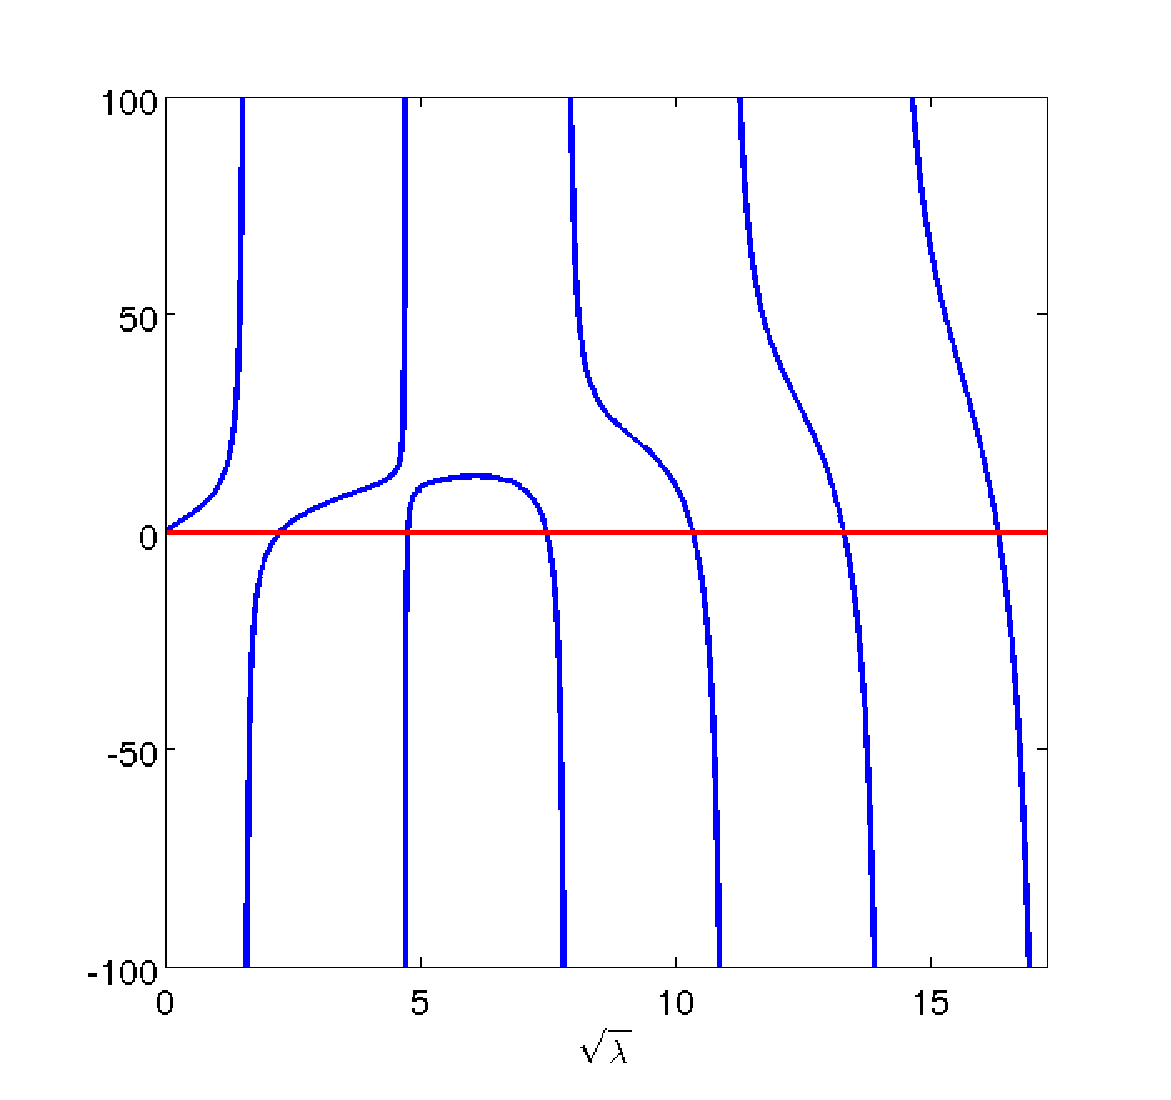
\includegraphics[scale=0.3]{Varie/ricercazeri}
\end{figure}
Esso sar\`a utilizzato da \texttt{EigensProvider()}, un complicato metodo della classe \classe{ModalSpace} che verr\`a descritto in seguito.

Vedremo che \classe{ModalSpace} possiede delle matrici per contenere la valutazione delle funzioni di base e delle loro derivate
nei nodi di quadratura sul quadrato riferimento.
Per riempire queste matrici \classe{ModalSpace} chiama i due metodi \texttt{EvaluateBasis()} dei generatori di base in direzione $y$ e $z$:
sono quelli infatti gli oggetti che conoscono la forma delle funzioni di base. 
Facendo riferimento alla forma generica delle basi modali \eqref{eq: 1sottoproblema} e alla tabella \ref{tab}, il compito di \texttt{EvaluateBasis()}
\`e di calcolare i coefficienti A e B in modo tale che le basi rispettino le condizioni di bordo e risultino normali ( ricordiamo che 
l'ortogonalit\`a \`e garantita dalla teoria ).

La registrazione delle valutazioni della base modale nei nodi di quadratura \`e necessaria per velocizzare le operazioni di 
integrazione evitando di valutarle ogni volta nuovamente.
Il metodo \texttt{EvalSinglePoint()} \`e stato aggiunto per valutare la funzione di base in un singolo punto.
Questa funzione si \`e resa necessaria in fase di export quanto desideravamo 
valutare la soluzione su una griglia 3D diversa da quella di quadratura.
\begin{figure}[!htbp]
        \centering%
        {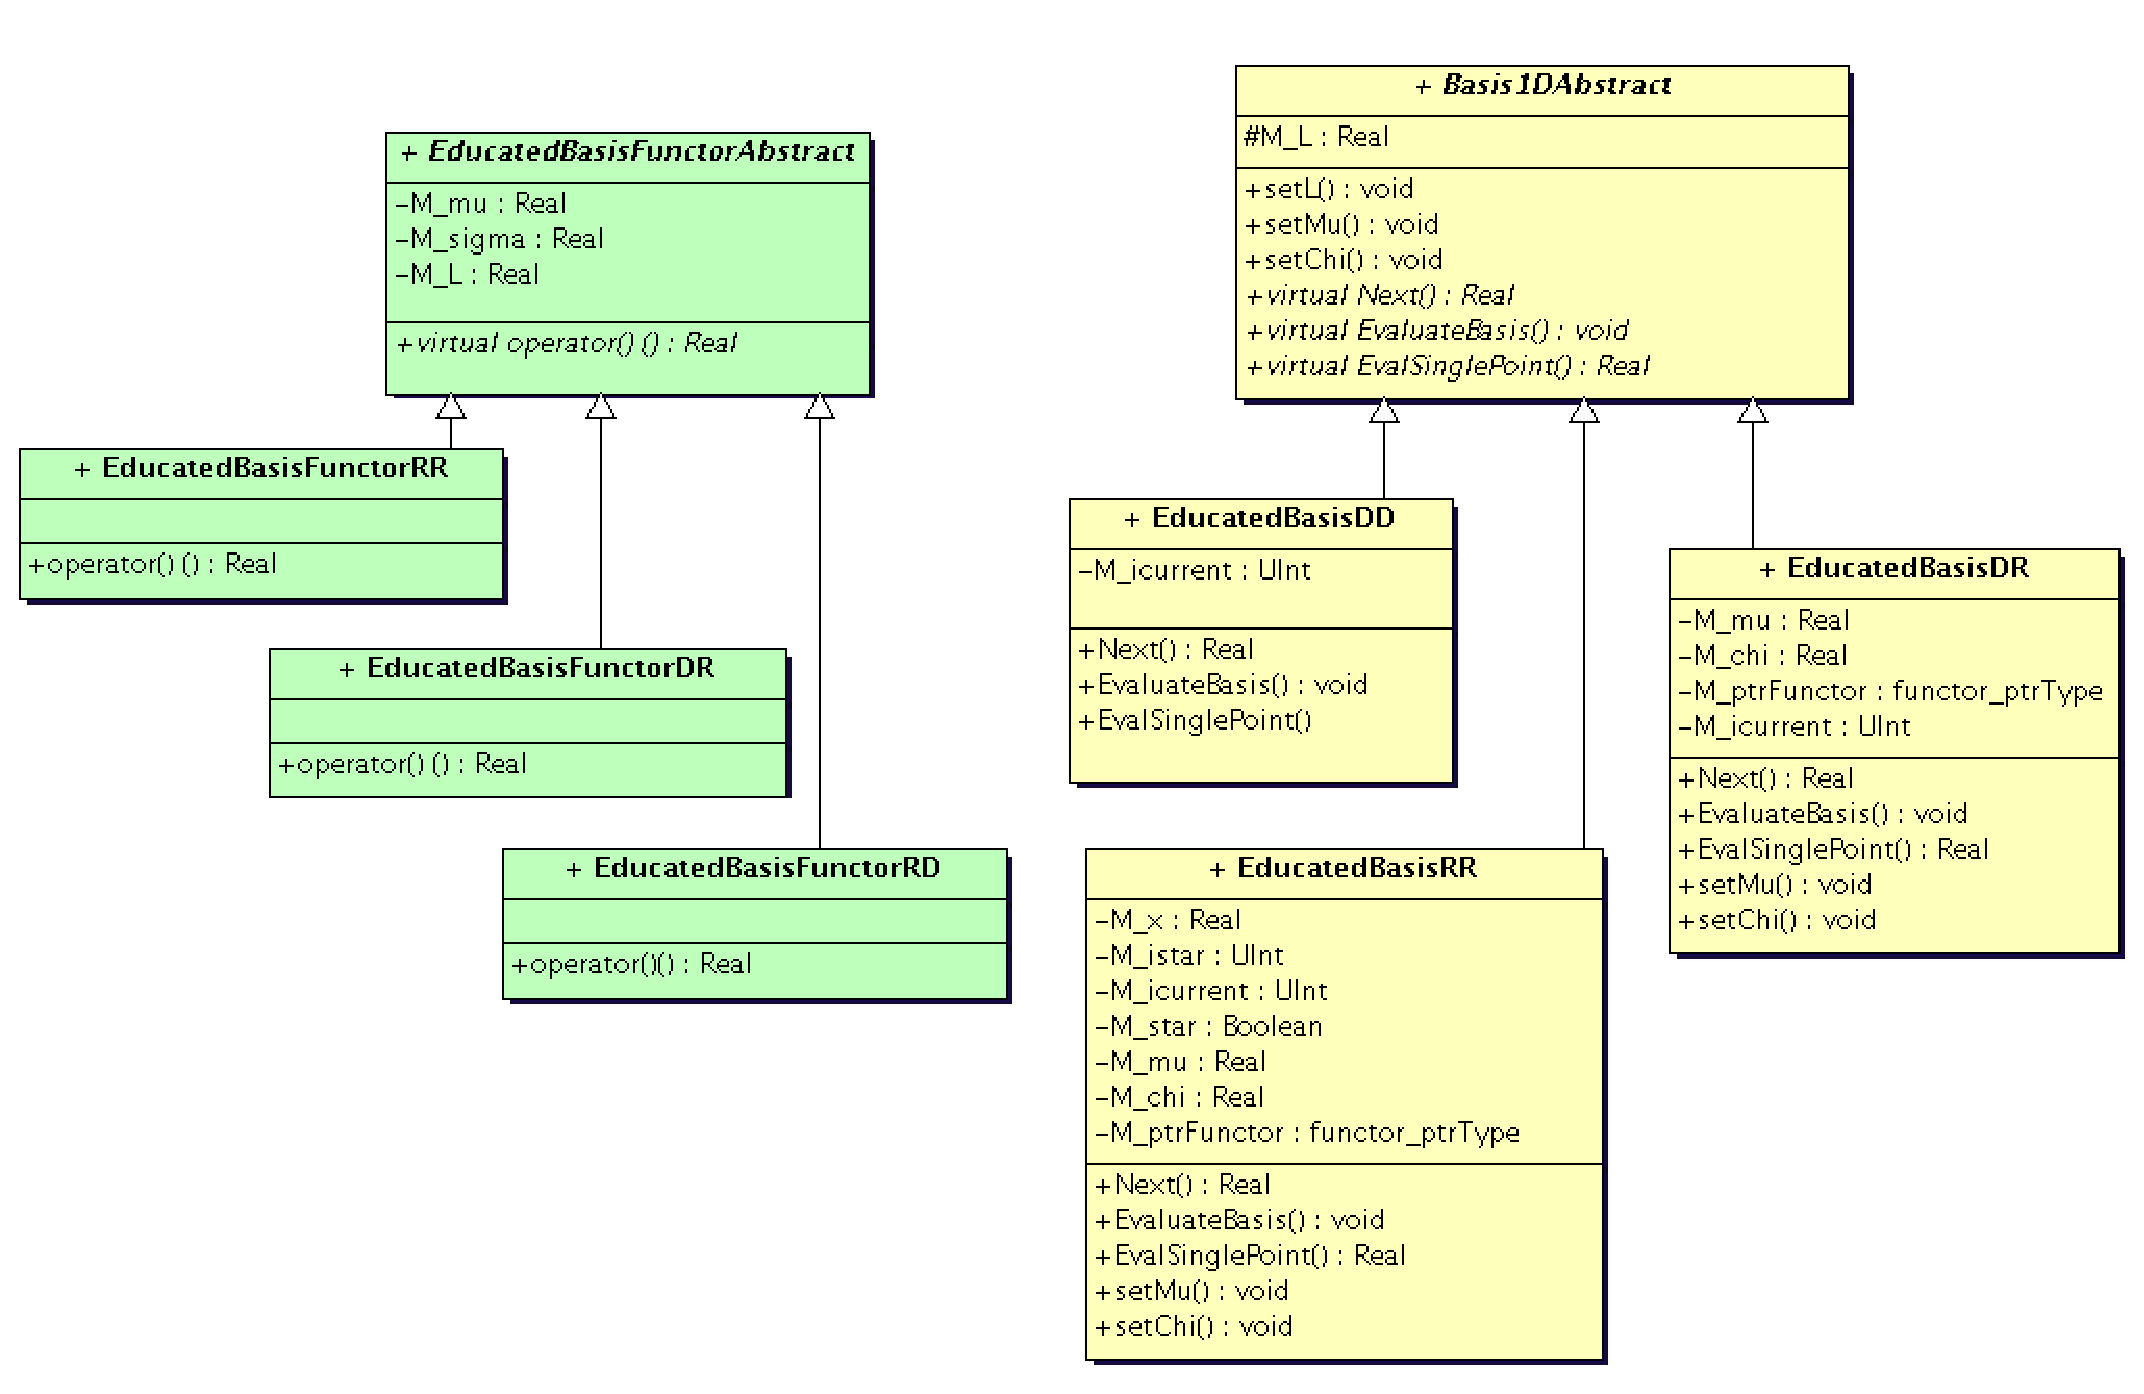
\includegraphics[scale=0.33]{UML/Basis1DAbstract.eps}}\qquad
        \caption{Classi Basis1DAbstract e EducatedBasisFunctor}
        \label{fig: UMLBasis}
\end{figure}
In figura \ref{fig: UMLBasis} riportiamo una descrizione grafica delle strutture dati appena presentate.

\section{Modalspace}
\classe{ModalSpace} \`e la classe che si occupa di utilizzare i due puntatori a \classe{Basis1DAbstract}.
Tramite questi oggetti \`e in grado di calcolare gli autovalori del problema 2D e, successivamente,
fornisce diversi metodi per l'integrazione sulla slice e per il calcolo dei coefficienti di Fourier.
Inizialmente \classe{ModalSpace} era stata concepita per essere una classe base, 
dalla quale fosse possibile ereditare ogni possibile scelta delle condizioni al bordo laterale, senza utilizzare \classe{Basis1DAbstract}. 
Tuttavia facendo un rapido conto ci siamo resi conto che, per implementare tutte le diverse combinazioni di condizioni 
di Dirichlet, Neumann e Robin sui lati della sezione rettangolare, arriviamo a ottantuno possibili combinazioni, 
una grande quantit\`a di codice da scrivere, che comprende casistiche molto simili fra loro se non identiche. 
Abbiamo dunque deciso di scorporare la gestione delle condizioni di bordo dalla classe \classe{ModalSpace}, 
per poi includerlo in modo ottimale in \classe{Basis1DAbstract}. 
Un secondo punto a favore di questa scelta riguarda la valutazione e la lettura delle basi modali.
Se avessimo scelto di adottare l'ereditariet\`a in ModalSpace, ogni eventuale 
figlia avrebbe avuto un tipo di base differente e accedervi tramite la classe base ogni qual volta 
fosse necessario, poteva essere inefficiente. \classe{ModalSpace} contiene le valutazioni delle basi modali e delle derivate 
su un'opportuna griglia di quadratura, i generatori di basi, diversi metodi di integrazione sulle slice oltre all'algoritmo e alle strutture dati necessarie
per la gestione degli autovalori. Questo design, rispetto alla nostra scelta iniziale, attribuisce maggiore 
generalit\`a: \classe{ModalSpace} \`e pronta ad utilizzare qualunque tipo di base modale nella forma \classe{Basis1DAbstract}.

\subsection{Costruzione e setting}
\classe{ModalSpace} conosce la geometria della sezione (Ly, Lz) e deve conoscere il numero di modi da utilizzare, ossia il numero di funzioni di base sulla slice trasversale (mtot). 
Un altro parametro che si pu\`o settare nel costruttore \`e la regola di quadratura da utilizzare sulla slice. 
Si noti che le basi utilizzate necessitano regole di quadratura di alto ordine e il numero di nodi di quadratura necessario
\`e strettamente legato al numero di modi\footnote{Per chi fosse interessato a esplorare questo aspetto c'\`e un tutorial (\texttt{2\_check\_basis}) che approfondisce questa
tematica e consente di fare qualche test}.
Questo legame \`e evidente se si pensa che maggiore \`e il modo, 
maggiore sar\`a la frequenza della base modale e il numero delle sue oscillazioni. 

Nella sezione quadrata una buona approssimazione del numero di modi in ciascuna direzione \`e $\sqrt{mtot}$. Il risultato non \`e valido nel caso di sezioni 
molto asimmetriche, infatti rettangoli molto allungati in una direzione avranno bisogno di pi\`u modi lungo la direzione maggiore e meno 
sull'altra. Per testare qualitativamente la precisione dell'integrazione abbiamo calcolato $$\sum_{j=1}^m\sum_{i=1}^m 
\left|(\varphi_j\varphi_i)_{numerico}- \delta_{ji}\right|$$ e abbiamo riportato i valori nella tabella \ref{quad}.
Nella seconda colonna della tabella \`e riportato il massimo tra tutti i valori di $p,q$. Vediamo come questo valore cresca 
al crescere dello stretching della sezione: quando il dominio \`e molto allungato in una direzione tutti i modi vengono spesi
per approssimare il fenomeno in quella direzione, mentre nell'altra si user\`a solo la prima funzione di base (ad esempio q=1 p=$1\div mtot$).
In casi come questo la frequenza massima \`e altissima ed \`e dunque meglio utilizzare una regola di quadratura appropriata.
\begin{table}[h]
\centering
\begin{tabular}{|c|c|c|c|c|}
\hline
Lx&Ly & Max(p,q) &  32 nodi &  64 nodi \\
\hline
1.0&2.0 & 12 & 1.85391e-9 & 9.54883e-14 \\
\hline
1.0&4.0 & 16 & 8.7809e-4 & 1.51567e-13 \\
\hline
1.0&8.0 & 23 & 7.87756 & 2.70061e-13 \\
\hline
1.0&16.0 & 33 & 54.7566 & 7.91844e-6 \\
\hline
1.0&32.0 & 50 & 185.541 & 32.7153 \\
\hline
\end{tabular}
\caption{Qualit\`a dell'integrazione al variare della quadratura (mtot=50)}
\label{quad}
\end{table}

Una volta creato l'oggetto \texttt{ModalSpace} bisogna eseguire alcuni set importanti. Per prima cosa dobbiamo settare i generatori di base 
lungo le direzioni trasversali. Nel caso di basi istruite questa operazione viene fatta imponendo le condizioni al bordo laterale
tramite i metodi
\begin{itemize}
\item \texttt{void AddSliceBCY(const string\& left, const string\& right, const Real\& mu = 1, const Real\& Chi =1)};
\item \texttt{void AddSliceBCZ(const string\& left, const string\& right, const Real\& mu = 1, const Real\& Chi =1)}
\end{itemize}

\begin{lstlisting}[style = general]
void ModalSpace::
AddSliceBCY (const string& left, const string& right, const Real& mu, const Real& chi)
{
	M_genbasisY = Basis1DFactory::istance().createObject(left+right;)
	M_genbasisY->setL(M_Ly);
	M_genbasisY->setMu(mu);
	M_genbasisY->setChi(chi)
	return;
}
\end{lstlisting}
Questo metodo si preoccupa di costruire il generatore di base corretto a seconda delle richieste sulle condizioni al bordo.
In particolare abbiamo deciso di utilizzare una factory per gestire questo passaggio in maniera dinamica.
Tutte le classi figlie di \classe{Basis1DAbstract} devono essere caricate in una factory con un ID ragionevole.
Per le basi istruite gli ID hanno la forma $bc_{sinistra}$ + $bc_{destra}$, in questo modo
quando l'utente assegna le condizioni al bordo pu\`o essere completamente all'oscuro della struttura della basi monodimensionali e
della factory: \`e necessario solamente specificare la natura delle condizioni al bordo. Dopodich\`e il metodo setta opportunamente i parametri, nel caso di condizioni che non necessitino la definizione di $\chi$ o $\mu$
si pu\`o lasciare il default. Per utilizzare
il codice in versione 2D invece che 3D, basta specificare per una delle slice \emph{fake + basis}.


Infine si conlude il setting della classe \classe{ModalSpace} tramite la funzione membro pubblica \texttt{EvaluateBasis()}, 
che chiama le funzioni adibite a riempire le strutture dati che descriveremo successivamente.

Concludendo la parte relativa al setting, riportiamo le uniche linee di codice che l'utente dovr\`a scrivere nel 
main.
\begin{lstlisting}[style = general]
boost::shared_ptr<ModalSpace> MB (new ModalSpace(Ly,Lz,mtot,quadY,quadZ));
MB ->AddSliceBCY("dir","dir");
MB ->AddSliceBCZ("rob","rob",1.,3.);
MB ->EvaluateBasis();
\end{lstlisting}

\subsubsection{Strutture dati}
Diamo una breve descrizione delle strutture dati possedute dalla classe \classe{ModalSpace}. Prima di cominciare vorremmo 
ricordare che le basi modali sono calcolate sul quadrato di riferimento. Per non incorrere in errori fra dominio reale e riferimento,  
utilizzeremo la seguente notazione:
\begin{equation}
\label{eq: notazione}
\begin{array}{l l l}
\hat{\varphi}_j(\hat{y},\hat{z}) = \hat{\eta}_j(\hat{y}) \hat{\xi}_j(\hat{z}) & \hat{y} \in [0,1] & \hat{z} \in [0,1] 
\\
\\
\int_0^1 \hat{\eta}^2_j\,d\hat{y} = 1 & \int_0^1 \hat{\xi}^2_j\,d\hat{z} = 1
\end{array}
\end{equation}
Dove $\hat{\varphi_j}$ \`e la base modale ortonormale sul dominio di riferimento, risultato del prodotto delle basi ottenute tramite i 
generatori di basi.
Vediamo ora come gestire il passaggio dalle basi definite sul riferimento a quelle invece sul dominio reale. L'ortogonalit\`a si conserva 
facilmente, ma lo stesso discorso non vale per la normalizzazione. Verifichiamo che un semplice cambio di coordinate non conserva la 
normalizzazione:

\begin{equation}
\label{eq: trasformazione}
\begin{array}{l l }
\int_0^{L_y}\int_0^{L_z} \varphi_j(y,z)^2 \,dydz 
\\
\\
= \int_0^{L_y} \eta_j(y)^2 \,dy\int_0^{L_z} \xi_j(z)^2 \,dz 
\\
\\
= \int_0^{1} \eta_j(L_y\hat{y})^2 L_y\,d\hat{y} \int_0^{1} \xi_j(L_z\hat{z})^2 L_z\,d\hat{z} 
\\
\\
 = L_yL_z\int_0^{1} \hat{\eta}_j(\hat{y})^2 \,d\hat{y} \int_0^{1} \hat{\xi}_j(\hat{z})^2 \,d\hat{z} & \neq  1  
\end{array}
\end{equation}

Da questi passaggi deduciamo che per conservare la normalizzazione, la base che stiamo cercando avr\`a la seguente forma:
\begin{equation}
\label{eq: base sul dominio corrente}
\varphi_j(y,z) = (L_yL_z)^{-\frac{1}{2}}\hat{\eta}_j(yL_y^{-1})\hat{\xi}_j(zL_z^{-1})
\end{equation}
In conclusione, nei conti che verranno proposti si faccia sempre riferimento all'equazione \eqref{eq: base sul dominio corrente}.

Riconosciamo cinque strutture dati fondamentali per la classe \texttt{ModalSpace}:

\begin{itemize}

\item \texttt{M\_eigenvalues} contiene la mappa fra l'indice della base modale ($k$) e le sottofrequenze ($wp$ e $wq$) e i sottoindici corrispondenti ($p$ e $q$), viene prodotta in fase di setting dello 
spazio modale tramite la funzione membro \texttt{EigensProvider()}, chiamata da \texttt{EvaluateBasis()}. Il tipo \`e un \texttt{vector$<
$EigenMap$>$}.
 
\begin{lstlisting}[style = general]
struct EigenMap
{
	Real wp;	//subfrequency y
	Real wq;	//subfrequency z
	UInt p;
	UInt q;
	
	static EigenMap make_eigenmap(const Real& _wp,const Real& _wq,const UInt& _p,const UInt& _q)
	{
		EigenMap a;
		a.wp = _wp;
		a.wq = _wq;
		a.p = _p;
		a.q = _q;
		return a;	
	}
};
\end{lstlisting}
La componente k-esima del vettore contiene gli indici delle basi modali monodimensionali e le relative frequenze che sono associate agli autovalori
dei problemi monodimensionali.
L'ordinamento gerarchico degli autovalori e la corrispondenza delle sottofrequenze con i sottoindici sono fondamentali, approfondiremo in seguito 
il metodo \texttt{EigensProvider()}.

\item \textbf{MBMatrix\_type M\_phiy}, \`e un \texttt{vector$<$vector$<$Real$>$ $>$} che raccoglie la valutazione di $\hat{\eta}_j(\hat{y})$ $\forall j$ e per ogni nodo di quadratura lungo $\hat{y}\in[0,1]$.

\item \textbf{MBMatrix\_type M\_phiz}, \`e un \texttt{vector$<$vector$<$Real$>$ $>$} che raccoglie la valutazione di $\hat{\xi}_j(\hat{y})$ $\forall j$ e per ogni nodo di quadratura lungo $\hat{z}\in[0,1]$.

\item \textbf{MBMatrix\_type M\_dphiy}, \`e un \texttt{vector$<$vector$<$Real$>$ $>$} che raccoglie la valutazione di $\frac{\partial\hat{\eta}_j}{\partial 	\hat{y}}$ $\forall j$ e per ogni nodo di quadratura lungo $\hat{y}\in[0,1]$.

\item \textbf{MBMatrix\_type M\_dphiz}, \`e un \texttt{vector$<$vector$<$Real$>$ $>$} che raccoglie la valutazione di $\frac{\partial\hat{\xi}_j}{\partial 	\hat{z}}$ $\forall j$ e per ogni nodo di quadratura lungo $\hat{z}\in[0,1]$.

\end{itemize}
\subsection{\classe{EigensProvider()}}
 Abbiamo deciso di dedicare una sezione solamente a questo metodo, poich\'e la ricerca degli autovalori occupa un ruolo fondamentale nella 
struttura del codice.
 Il metodo viene chiamato da \texttt{EvaluateBasis()} dunque dopo che sono stati settati i generatori di basi. La funzione deve preoccuparsi di 
riempire la struttura dati \texttt{M\_eigenvalues}, tuttavia il procedimento non \`e semplice. 
 Per comprendere le difficolt\`a occorre ragionare sulla struttura del problema: separando le variabili lungo la slice 2D abbiamo ottenuto due 
problemi agli autovalori 1D (sezione \ref{sec: educated basis}). Ognuno di questi genera una successione ordinata crescente di autovalori, 
determinata dalla risoluzione del problema agli autovalori, che nel caso di basi istruite si traduce nella ricerca degli zeri di una data 
funzione, spesso, non lineare. Definiamo la successione di autovalori in $y$ con $\{K_y\}_p$ e quella in $z$ con $\{K_z\}_q$. Esse 
definiscono univocamente la successione degli autovalori del problema di partenza 2D e sono in relazione con essa nel seguente modo:

\begin{equation}
\label{eq: autovalori}
 \lambda_j = (K_y^p)^2 + (K_z^q)^2
\end{equation} 

Anche $\{\lambda\}_j$ \`e una successione crescente di autovalori, ma il suo ordinamento, dato quello dei sottoautovalori, non \`e immediato. 
Due sono le difficolt\`a che si presentano:
\begin{itemize}
\item[1.] Ogni sottoautovalore \`e il risultato di una ricerca di zeri di una funzione, spesso, non lineare.
\item[2.] L'utente stabilisce il numero massimo di modi sul problema 2D e non sui sotto-problemi 1D.
\end{itemize}

Le due problematiche sono strettamente legate, difatti non siamo interessati a cercare pi\`u sottoautovalori del necessario. Si poteva partire 
calcolando ad esempio 10 sottoautovalori in $y$ e altrettanti in $z$, combinarli in tutti i modi possibile ottenendo cento autovalori 2D
e poi ordinarli. Questo metodo ha due difetti: \`e poco efficiente ed inoltre pu\`o cadere in errore. Infatti l'algoritmo si dovrebbe fermare una volta 
raggiunti un numero di autovalori 2D pari ad \texttt{M\_mtot}, ma cos\`i facendo nessuno ci assicura che nel gruppo successivo di sottoautovalori,
una volta combinati a formare autovalori 2D, non se ne trovi uno minore dell'ultimo autovalore calcolato.

La soluzione \`e stata quella di procedere un passo alla volta, con l'accortezza di salvare i sotto-autovalori ancora non utlizzati. 
Il metodo \texttt{Next()} dei generatori fornisce progressivamente uno 
zero alla volta.

L'algoritmo \`e il seguente
\begin{enumerate}
 \item Inserire in fondo al vettore degli autovalori 2D (Eigenvalues), al primo posto, la coppia fatta dal pi\`u piccolo autovalore di entrambi i sottoproblemi ( $p=1,q=1$ )
 \item Calcolare gli autovalori 1D successivi  per entrambi i sottoproblemi e inserire gli autovalori 2D associati alle coppie $(p=2,q=1)$,$(p=1,q=2)$
 in un \texttt{set} (tmp) ordinato secondo un'opportuna relazione d'ordine che ci consente di evitare doppioni e di avere sempre in cima il pi\`u 
 piccolo autovalore 2D.
 \item Estrarre da tmp la coppietta $(\bar p,\bar q)$ in testa ( associata dunque all'autovalore 2D pi\`u piccolo) e inserirla nella lista degli autovalori 2D.
 \item Calcolare gli autovalori 1D associati $\bar p +1$ e a $\bar q+1$, inserire i due nuovi autovalori 2D associati a $(\bar p+1,\bar q)$ e $(\bar p,\bar q+1)$ in tmp.
 \item Ripetere il punto 3 fino a trovare \texttt{M\_mtot} autovalori 2D.
\end{enumerate}

Alcune accortezze sono state prese per evitare di calcolare pi\`u volte gli stessi autovalori. La relazione d'ordine \`e stata scelta con estrema
cura per poter considerare autovalori 2D con molteplicit\`a algebrica maggiore di uno, questi autovalori infatti devono essere inseriti in tmp perch\'e
non sono doppioni.
\begin{lstlisting}[style = general]
bool Comparison::
operator() (const EigenMap& a, const EigenMap& b) const
{
//Se le coppiette non sono associate allo stesso autovalore 2D
if ( ( pow (a.wp, 2) + pow (a.wq, 2) ) != ( pow (b.wp, 2) + pow (b.wq, 2) ) ) 
{
  //Restituisci la coppietta associata all'autovalore 2D piu' piccolo
  return (pow (a.wp, 2) + pow (a.wq, 2) ) < (pow (b.wp, 2) + pow (b.wq, 2) ); 
}
else
{
  //Se l'autovalore 2D e' lo stesso restituisci quello con la frequenza in direzione y minore, in questo modo, se e' un doppione, verra' riconosciuto in quanto ne maggiore ne minore
  return a.wp < b.wp ; 
}
}
\end{lstlisting}
Proviamo a dare una visualizzazione dell'algoritmo.

\begin{tikzpicture}[stack/.style={
  rectangle split, rectangle split parts=5, draw, anchor=center},
  myarrow/.style={single arrow, draw=none}]

\node [stack] (prima)  {\nodepart{two}
\nodepart{three}\nodepart{four}
\nodepart{five}$Ky^{(1)},Kz^{(1)}$};

\node [stack,right=of prima] (seconda) {\nodepart{two}
  \nodepart{three}\nodepart{four}$Ky^{(1)},Kz^{(2)}$
  \nodepart{five}$Ky^{(2)},Kz^{(1)}$};

\node [stack,right=of seconda] (terza) {{\nodepart{two}
\nodepart{three}\nodepart{four}$Ky^{(2)},Kz^{(1)}$
\nodepart{five}$Ky^{(1)},Kz^{(1)}$};

\node [stack,right=of terza] (quarta) {\nodepart{two}
  \nodepart{three}\nodepart{four}
  \nodepart{five}$Ky^{(1)},Kz^{(2)}$};
  
\node [above=of prima,anchor=north,align=left] {Eigenvalues};
\node [above=of seconda,anchor=north,align=left] {Tmp};
\node [above=of terza,anchor=north,align=left] {Eigenvalues};
\node [above=of quarta,anchor=north,align=left] {Tmp};

\node [myarrow,draw,anchor=west] at ($(seconda.east)+(2.5pt,0)$) {\phantom{te}} ;

%\node [myarrow,draw,anchor=west] at ($(mid.east)+(2.5pt,0)$) %{\phantom{te}} ;
\draw [red,ultra thick,->] ($(seconda.west)+(-0.1,-1.0)$) -- ($(prima.east)+(0.1,-0.4)$);
\draw [red,thick] ($(seconda.south)+(-1.4,-0.2)$)--($(seconda.south)+(1.4,0.8)$);
\draw [red,thick] ($(seconda.south)+(-1.4,0.8)$)--($(seconda.south)+(1.4,-0.2)$);
 % {instruction 0;\\ instruction 1;\\$\ldots$\\instruction $n$;};
\end{tikzpicture}
%\begin{tikzpicture}
%[scale=1.5]
%\tikzstyle{every node}=[draw,shape=rectangle];
%\path (5,0)   node (v1) {$Ky^{(1)},Kz^{(1)}$};
%\path (3,-1) node (v2) {$Ky^{(2)},Kz^{(1)}$};
%\draw (v1) -- (v2);
%\end{tikzpicture}

\begin{tikzpicture}[stack/.style={
  rectangle split, rectangle split parts=5, draw, anchor=center},
  myarrow/.style={single arrow, draw=none}]

\node [stack] (prima) {{\nodepart{two}
  \nodepart{three}\nodepart{four}$Ky^{(2)},Kz^{(1)}$
  \nodepart{five}$Ky^{(1)},Kz^{(1)}$};

\node [stack,right=of prima,rectangle split part fill={white,white,blue!20,blue!20,white}] (seconda) {\nodepart{two}\textcolor{blue!100}{New}
  \nodepart{three}$Ky^{(2)},Kz^{(2)}$\nodepart{four}$Ky^{(3)},Kz^{(1)}$
  \nodepart{five}$Ky^{(1)},Kz^{(2)}$};
  
  \node [stack,right=of seconda] (terza)  {\nodepart{two}
\nodepart{three}$Ky^{(1)},Kz^{(2)}$\nodepart{four}$Ky^{(2)},Kz^{(1)}$
\nodepart{five}$Ky^{(1)},Kz^{(1)}$};

\node [stack,right=of terza] (quarta) {\nodepart{two}
  \nodepart{three}\nodepart{four}$Ky^{(2)},Kz^{(2)}$
  \nodepart{five}$Ky^{(3)},Kz^{(1)}$};
  
\node [above=of prima,anchor=north,align=left] {Eigenvalues};
\node [above=of seconda,anchor=north,align=left] {Tmp};
\node [above=of terza,anchor=north,align=left] {Eigenvalues};
\node [above=of quarta,anchor=north,align=left] {Tmp};

\node [myarrow,draw,anchor=west] at ($(seconda.east)+(2.5pt,0)$) {\phantom{te}} ;

\draw [red,ultra thick,->] ($(seconda.west)+(-0.1,-1.0)$) -- ($(prima.east)+(0.1,+0.1)$);
\draw [blue,dashed,ultra thick,->] ($(prima.east)+(0.1,-0.3)$) -- ($(seconda.west)+(-0.1,+0.1)$);
\draw [blue,dashed,ultra thick,->] ($(prima.east)+(0.1,-0.3)$) -- ($(seconda.west)+(-0.1,-0.5)$);
\draw [red,thick] ($(seconda.south)+(-1.4,-0.2)$)--($(seconda.south)+(1.4,0.8)$);
\draw [red,thick] ($(seconda.south)+(-1.4,0.8)$)--($(seconda.south)+(1.4,-0.2)$);
%\node [myarrow,draw,anchor=west] at ($(mid.east)+(2.5pt,0)$) %{\phantom{te}} ;
%\draw [align=left,above=of seconda,label=above:{New}] ($(seconda.south)+(-1.2,0.8)$) rectangle ($(seconda.south)+(1.2,2)$);
 % {instruction 0;\\ instruction 1;\\$\ldots$\\instruction $n$;};
\end{tikzpicture}
%\begin{tikzpicture}
%[scale=1.5]
%\tikzstyle{every node}=[draw,shape=rectangle];
%\path (5,0)   node (v1) {$Ky^{(1)},Kz^{(1)}$};
%\path (3,-1) node (v2) {$Ky^{(2)},Kz^{(1)}$};
%\path (7,-1) node (v3) {$Ky^{(1)},Kz^{(2)}$};
%\draw (v1) -- (v2)
%(v1) -- (v3);
%\end{tikzpicture}

\vspace{1cm}

\begin{tikzpicture}
[scale=1.5]
\tikzstyle{every node}=[draw,shape=rectangle];
\path (5,0)  node (v1) {$Ky^{(1)},Kz^{(1)}$};
\path (3,-1) node (v2) {$Ky^{(2)},Kz^{(1)}$};
\path (7,-1) node (v3) {$Ky^{(1)},Kz^{(2)}$};
\path (2,-2) node (v4) {$Ky^{(3)},Kz^{(1)}$};
\path (4,-2) node (v5) {$Ky^{(2)},Kz^{(2)}$};
\path (6,-2) node (v6) {$Ky^{(2)},Kz^{(2)}$};
\path (8,-2) node (v7) {$Ky^{(1)},Kz^{(3)}$};
\draw (v1) -- (v2)
(v1) -- (v3)
(v2) -- (v4)
(v2) -- (v5)
(v3) -- (v6)
(v3) -- (v7);
\draw [thick,red, -] (5.5,-1.5)--(6.5,-2.5);
\draw [thick,red, -] (6.5,-1.5)--(5.5,-2.5);
\end{tikzpicture}

In questo albero rappresentiamo come si effettua la ricerca e vediamo che il nodo con la x rossa \`e stato
cancellato perch\'e \`e un doppione.
Ogni nodo rappresenta un coppietta di sotto autovalori. Ogni volta che un nuovo autovalore viene
inserito nella lista di eigenvalues, i suoi due nodi figli vengono inseriti nell'albero.
A ogni iterazione tmp contiene tutte le foglie, ordinate in base al valore dell'autovalore 2D associato, e si 
occupa anche di non inserire nell'albero i doppioni.



\subsection{Metodi di calcolo}
Approfondiamo ora i metodi che si occupano di calcolare i coefficienti della matrice di sistema.

\begin{itemize}
\item \texttt{Real Compute\_PhiPhi(const UInt\& j, const UInt\& k)}

 $\int_{\gamma}\varphi_j(y,z)\varphi_k(y,x) \,dydz$

\item \texttt{Real Compute\_DyPhiPhi(const UInt\& j,const UInt\& k)} 

$\int_{\gamma} \partial_y \varphi_j(y,z)\varphi_k(y,x) \,dydz$

\item \texttt{Real Compute\_DzPhiPhi(const UInt\& j,const UInt\& k)} 

$\int_{\gamma} \partial_z \varphi_j(y,z)\varphi_k(y,x) \,dydz$

\item \texttt{Real Compute\_DyPhiDyPhi(const UInt\& j,const UInt\& k)} 

$\int_{\gamma} \partial_y \varphi_j(y,z)\partial_y\varphi_k(y,x) \,dydz$

\item \texttt{Real Compute\_DzPhiDzPhi(const UInt\& j,const UInt\& k)} 

$\int_{\gamma} \partial_z \varphi_j(y,z)\partial_z\varphi_k(y,x) \,dydz$

\item \texttt{Real Compute\_Phi(const UInt\& k)} 

$\int_{\gamma} \varphi_k(y,x) \,dydz$

\item \texttt{vector$<$Real$>$ FourierCoefficients (const function\_Type\& g) const},

data una funzione indipendente da $x$ questo metodo restituisce i coefficienti di Fourier (in numero pari ad \texttt{M\_mtot}) rispetto alla base modale scelta.

\item \texttt{Real FourierCoeffPointWise (	const Real\& x,const function\_Type\& f,const UInt\& k ) const},

restituisce il $k$-esimo coefficiente di Fourier di una generica funzione 3D rispetto alla base modale una volta fissato un punto $x$.
\end{itemize}

Vediamo come esempio l'implementazione di \texttt{Compute\_PhiPhi()}:

\begin{lstlisting}[style = general]
Real ModalSpace::
Compute_PhiPhi(const UInt& j, const UInt& k) const
{
	Real coeff_y = 0.0;
	Real coeff_z = 0.0;
	UInt p_j = M_eigenvalues[j].p-1;
	UInt p_k = M_eigenvalues[k].p-1;
	UInt q_j = M_eigenvalues[j].q-1;
	UInt q_k = M_eigenvalues[k].q-1;
	
	Real normy = 1.0 / sqrt(M_Ly);
	Real normz = 1.0 / sqrt(M_Lz);
	
	for(UInt n = 0; n < M_quadruleY->nbQuadPt();++n)
	{
		coeff_y +=	M_phiy[p_j][n] * normy *	
							M_phiy[p_k][n] * normy *
							M_Ly * M_quadruleY->weight(n);
	}
	
		for(UInt n = 0; n < M_quadruleZ->nbQuadPt();++n)
	{
		coeff_z +=	M_phiz[q_j][n] * normz *	
							M_phiz[q_k][n] * normz *
							M_Lz * M_quadruleZ->weight(n);
	}
	
	return coeff_y*coeff_z;
}
\end{lstlisting}
 L'implementazione \`e basata sulla separazione di variabili, nel caso di coefficienti non costanti bisogner\`a cambiare
 questa implementazione.
 I metodi per calcolare i coefficienti di Fourier sono indispendabili 
 ed il loro impiego sar\`a pi\`u chiaro una volta vista la classe \classe{HiModAssembler}.
 
\section{HiModAssembler}
 
 In questa classe viene gestita la fase di assemblaggio del problema e quella di export. Abbiamo cercato di seguire la linea della classe 
FESpace, infatti \texttt{HiModAssembler} \`e templetizzata sugli stessi argomenti. 

 \begin{lstlisting}[style = general]
 template<typename mesh_type,typename matrix_type,typename vector_type>
 class HiModAssembler
 {
	... 
 };
 \end{lstlisting} 
Oltre a mantenere una struttura di base coerente con lo 
spazio agli elementi finiti, la scelta di templetizzare le matrici e i vettori, manipolati da tale classe, prevede una possibile estensione a strutture algebriche pi\`u adatte al metodo di riduzione gerarchica. 
 
 Viene templetizzata anche la mesh, ma questo parametro si riferisce discretizzazione della fibra di supporto, dunque siamo vincolati a 
trattarlo in questo modo.
 Momentanemante il codice funziona solamente con strutture algebriche del tipo EpetraStructured, tuttavia occorrerebbe ripensare attentamente questa parte, 
soprattutto in vista di una possibile parallelizzazione.
Un codice HiMod ottimizzato dovr\`a possedere delle proprie strutture, adeguate al pattern della matrice di sistema.


 
\subsubsection{I membri}
La classe HiModAssembler posside tre membri privati:

\begin{itemize}
\item \texttt{modalbasis\_ptrType M\_modalbasis
\item \texttt{fespace\_ptrType M\_fespace
\item \texttt{etfespace\_ptrType M\_etfespace}}}
\end{itemize}

Nota la teoria era chiaro che la classe dovesse possedere lo spazio modale 2D e lo spazio elementi finiti 1D.
Il restante oggetto esiste per una scelta di programmazione. Infatti abbiamo deciso di ricorrere all'utilizzo del pacchetto \texttt{ETA}, 
piuttosto che del \texttt{GeneralAssembler}. Due sono le motivazioni che hanno condotto a questa scelta:
\begin{itemize}
\item[1.] Semplicit\`a di scrittura della forma variazionale.
\item[2.] Possibilit\`a di scrivere pi\`u parti di forma variazionale.
\end{itemize}

Entrambe le motivazioni sono legate in realt\`a a possibili future estensioni del codice. Se pensiamo al problema generalizzato ad una qualunque 
sezione 2D, siamo costretti ad adottare una mappa che leghi lo spazio reale e lo spazio di riferimento (dove viene risolto il problema) si veda \cite{perotto:2008}. I conti 
mostrano che alla forma variazionale si aggiungono alcuni casi non gestiti dal \texttt{GeneralAssembler}.

L'utilizzo del modulo \texttt{ETA} \`e tuttavia nascosto all'utente, il costruttore si occupa di inizializzare \texttt{M\_etfespace} ricavando 
le informazioni necessarie da \texttt{M\_fespace}.
Lo spazio elementi finiti viene comunque conservato per alcune sue utility non presenti in ETFespace di cui avevamo bisogno.
\begin{lstlisting}[style=general]
 template<typename mesh_type,typename matrix_type,typename vector_type>
 HiModAssembler<mesh_type, matrix_type,vector_type>::
 HiModAssembler(	const fespace_ptrType& fespace,
 									const modalbasis_ptrType& modalbasis,
 									commPtr_Type& Comm):
 		M_Modalbasis	( modalbasis),
 		M_etfespace 	( new etfespace_type (fespace->mesh(),
 																 &(fespace->refFE()),
 																 &(fespace->fe().geoMap()),
 																 Comm))
		M_fespace		( fespace)
{} 																 
 																
\end{lstlisting}

\subsection{I metodi}
Proponiamo di seguito una descrizione dei vari metodi disponibili nella classe \texttt{HiModAssembler}. La classe \`e ampia, tuttavia comprende 
tre sezioni ben distinte: assemblaggio, analisi e export.
\subsubsection{Assemblaggio}
\begin{lstlisting}[style=general,frame=none]

void AddADRProblem	( const matrix_ptrType& systemMatrix,
											const Real& mu, 
											const TreDvector_type& beta, 
											const Real& sigma)
\end{lstlisting}
Si occupa dell'assemblaggio della matrice di sistema. I coefficienti sono considerati costanti, l'estensione 
a coefficienti non costanti comporta cambiamenti anche nella classe \texttt{ModalSpace}, tali modifiche non sono state apportate perch\`e esuliano
dai nostri obbiettivi progettuali. Si \`e ragionato su una possibile implementazione che segua la linea generale proposta nel report \citep{perotto:2008} \footnote{Nel caso si fosse interessati all'implementazione parte del codice \`e gi\`a presente nel branch \texttt{20130710\_HiModMap}}.
Le fasi di assemblaggio sono semplici: la matrice di sistema viene percorsa a blocchi e per ognuno di essi il computo dei valori avviene tramite 
il metodo \texttt{integrate} del pacchetto \texttt{ETA}. Difatti ogni blocco corrisponde al problema 1D che accoppia ldue frequenze.

\begin{lstlisting}[style = general, frame = none]

void interpolate	( const function_Type& f,
										const vector_ptrType& f_interpolated)
\end{lstlisting}
Data una generica funzione spaziale, questo metodo si occupa di calcolare, per ogni punto della griglia 1D, tutte le componenti di Fourier 
rispetto alle basi modali. Il risultato viene salvato nel vettore strutturato passato negli argomenti. \`E in questo punto che ricopre un ruolo 
fondamentale il metodo \texttt{FourierCoeffPointWise()} posseduto da \classe{ModalSpace}.
Calcolare le componenti di una generica funzione $H^1$ rispetto allo spazio del metodo HiMod  richiede prima una proiezione lungo le basi modali e successivamente un'interpolazione dei coefficienti di Fourier nello spazio elementi finiti. Le dimensioni del vettore che contiene le componenti della funzione sono pari ovviamente a \texttt{Mtot$\cdot$DOFfem}.

\begin{lstlisting}[style=general, frame = none]

void Addrhs	(	const vector_ptrType& rhs,
							const vector_ptrType& f_interpolated);
\end{lstlisting}
Definito il metodo \texttt{interpolate} risulta semplice assemblare il termine noto. Ottenuta l'interpolazione della forzante l'approccio non 
\`e differente da \texttt{AddADRProblem()}: il vettore \texttt{rhs} possiede \texttt{M\_mtot} blocchi di dimensione ciascuno pari ai gradi di 
libert\`a FEM, si scorrono tutti i blocchi e poich\`e ognuno di essi \`e legato al problema 1D riferito alla \texttt{j-esima} frequenza, il 
metodo \texttt{integrate()} computa gli opportuni coefficienti.

Mostriamo in breve le operazioni eseguite nel main per definire ed assemblere il termine noto:
\begin{lstlisting}[style = general,frame=bottomline]
boost::shared_ptr<vector_Type> rhs 
		(new vector_Typer (Map,Repated));
*rhs *= 0.0;
rhs -> setBlockStructure(block_row);

boost::shared_ptr<vector_Type> f_interpolated 
		(new vector_Type (Map,Repeated));

HM.interpolate ( f,f_interpolated );
HM.Addrhs (rhs,f_interpolated);
\end{lstlisting}

\begin{lstlisting}[style = general,frame = none]

void AddDirichletBC_In (	const matrix_ptrType& systemMatrix,
													const vector_ptrType& rhs,
													const function_Type& g)
\end{lstlisting}

L'applicazione delle condizioni di inflow ed outflow sono un aspetto secondario di questo lavoro, tuttavia non possono certo essere esenti da 
un'adeguata trattazione. Per quanto riguarda le condizioni naturali del problema \`e sufficiente intervenire nella forma variazionale, nel caso 
invece di condizioni essenziali quali quelle di Dirichlet, abbiamo deciso di intervenire con una penalizzazione algebrica, molto simile al 
trattamento delle BC fatto da FreeFem++. Per capire dove intervenire dobbiamo rifarci all'interpretazione data nei cenni teorici, ricordiamo 
infatti che la matrice di sistema del metodo HiMod \`e costituita da $\texttt{M\_mtot}^2$ problemi 1D correlati fra loro. Dunque se ogni 
sottoblocco rappresenta la matrice di sistema di un problema ADR agli elementi finiti 1D, \`e chiaro che sar\`a sufficiente intervenire sul 
primo elemento (nel caso di Dirichlet all'inflow) di ogni sottoblocco diagonale. Analogamente l'intervento sul termine noto, viene eseguito sostituendo al primo elemento di 
ogni sottoblocco, il coefficiente 
di Fourier del dato in ingresso, moltiplicato per il medesimo coefficiente di penalizzazione usato nella matrice di sistema. Otteniamo dunque che:
\begin{equation}
\label{eq: inflow}
\tilde u_k(0)=\tilde g_k \quad \forall k = 1 \ldots m_{tot}
\end{equation}

dove $\tilde g_k$ \`e il $k$-esimo coefficiente di Fourier del dato all'inflow $g(y,z)$.
Per calcolarli \`e stato sviluppato 
il metodo \texttt{FourierCoefficients()} contenuto in \texttt{ModalSpace}.
\clearpage
\subsubsection{Analisi}

I seguenti metodi si occupano di manipolare le informazioni contenute nel vettore soluzione o in un generico vettore dello spazio HiMod. Il nostro primo interesse \`e poter ricostruire i valori della soluzione nei punti della griglia 
3D costituita dai nodi di quadratura e i nodi FEM. Il vettore ottenuto sar\`a poi utilizzato per eventuali operazioni o analisi quali computo 
della norma L2.
Per eseguire confronti con generiche funzioni, abbiamo implementato anche una specializzazione nel caso l'argomento di ingresso risulti essere 
una generica funzione spaziale.

Ai fini di proporre confronti e grafici di convergenza \`e stata implementato il computo della norma L2.

\begin{lstlisting}[style = general,frame=none]

vector_type evaluateBase3DGrid (const vector_type& fun)

vector_type evaluateBase3DGrid (const function_Type& fun)

Real normL2 (const vector_type& fun)

\end{lstlisting}

La particolarit\`a dei metodi appena presentati \`e il fatto che non viene valutata nessuna funzione di base, si tratta solamente di recuperare i valori 
memorizzati nelle strutture dati di \texttt{M\_modalspace}. Tuttavia questo vantaggio \`e preservato fin tanto ci si accontenta di valutare la 
funzione nei punti della griglia di quadratura. Nel caso di una valutazione pi\`u fitta o di un punto arbitrario, occorre risalire alla forma 
originale delle basi modali. Questo \`e concesso grazie al metodo \texttt{EvalSinglePoint()}, posseduto da ogni generatore di basi il quale 
conosce la forma originale della base modale. Ovviamente tale approccio si poteva 
adottare anche per i precedenti metodi, ma l'utilizzo avrebbe comportato la valutazione di una funzione, posseduta da un oggetto posto nelle 
foglie di una struttura polimorfica. Il risultato finale sarebbe stato un costo computazionale notevolmente maggiore.


\subsubsection{Export}

L'export di un generico vettore dello spazio HiMod viene gestito dal metodo \texttt{ExporterStructuredVTK()}. Poich\`e  per sua natura la classe HiMod non possiede una griglia 3D,  il metodo ne genera una di supporto su cui eseguire l'export. 
L'operazione occupa molto tempo, infatti su ogni punto della mesh fittizia, 
occorre sommare i contributi di ogni frequenza del sistema. 
Inoltre questo valore deve essere moltiplicato per il valore assunto dalle basi FEM 1D in quel punto (nel caso P1 sono soltanto due).
Abbiamo scelto di ciclare prima sulle frequenze del sistema: per ogni modo vengono registrati 
tutti i contributi della funzione di base sulla slice (richiamando il metodo \texttt{EvalSinglePoint()}) 
e, successivamente, si cicla sui nodi della griglia, componendo le basi FEM, il vettore HiMod e 
i valori appena registrati della base modale.

\begin{lstlisting}[style = general,frame=none]
void ExporterStructuredVTK (	const UInt& nx,
															const UInt& ny,
															const UInt& nz,
															const vector_ptrType& fun,
															const GetPot& dfile, 
															string prefix,
															string content)
\end{lstlisting}

Nell'implementazione di questo metodo ci siamo focalizzati
solamente sulla valutazione della soluzione su una griglia, il metodo si appoggia, poi, sulla classe ExporterVTK.
Abbiamo poi implementato un metodo analogo per esportare sulla medesima griglia strutturata una generica funzione scalare.

\begin{lstlisting}[style = general,frame=none]
void ExporterFunctionVTK (	const UInt& nx,
															const UInt& ny,
															const UInt& nz,
															const function_Type& fun,
															const GetPot& dfile, 
															string prefix,
															string content)
\end{lstlisting}

Infine abbiamo implementato un'utitli\`a che potrebbe rivelarsi utile in futuro, 
ovvero una funzione che valuta un vettore appartenente allo spazio HiMod  su un generico punto appartentente ad $\Omega$.

\begin{lstlisting}[style = general,frame=none]
Real evaluateHiModFunc(const vector_ptrType& fun, const Real& x, const Real& y, const Real& z)
\end{lstlisting}
\clearpage
\chapter{Risultati}
In questa sezione mostreremo alcuni dei risultati che abbiamo ottenuto, per visualizzarli abbiamo utilizzato
il software ParaView.
All'interno del file \texttt{himod/util/CaseTest.hpp} sono salvati diversi casi test
con soluzione esatta e uno senza (la forzante \`e stata ottenuta usando il symbolic toolbox di Matlab).
Nel caso si fosse interessati ad aggiungere altri casi test \`e possibile aggiungerli modificando i
file \texttt{CaseTest.hpp} e \texttt{CaseTest.cpp}. Una volta creato il caso test 
occorre aggiungerlo allo switch che si trova nella classe \classe{GeneralTest} nella
cartella \texttt{util}. \classe{GeneralTest} \`e una classe che abbiamo sviluppato per poter
lanciare diversi test senza dover modificare il sorgente, ma semplicimente settando 
parametri  e caso test dal datafile di \texttt{GetPot}\footnote{Se si vuole provare a lanciare qualche test si veda il tutorial
\texttt{4\_generaltest}, se invece si vuole vedere come si dovrebbe assemblare un test da zero si veda il tutorial \texttt{1\_ADR} }.
Cominciamo mostrando il caso test senza soluzione esatta, che per\`o \`e pi\`u interessante dal punto di vista qualitativo.
\begin{equation}
 \label{eq:camini}
 \left\{
\begin{aligned}
 &-\Delta u + \vect{\beta}\cdot\nabla u + \sigma u = f &\quad \text{ in }\Omega=(0,2)\times(0,1)\times(0,1)\\
 &u=0 &\quad \text{ su } \Gamma_{in} \cup \Gamma_{lat}\\
 &\nabla u\cdot \vect{n} = 0 &\quad \text{ su } \Gamma_{out},
\end{aligned}
\right.
\end{equation}

dove $\vect{\beta}=(5,1,0)$, $\sigma=0.3$ e $f$ \`e riportata in figura \ref{fig:fcamini} e rappresenta due sorgenti 
di forma sferica.
In figura \ref{fig:confrontocamini} abbiamo in alto la soluzione ottenuta con
gli elementi finiti (sempre con LifeV), utilizzando una griglia strutturata con 20 elementi in direzione $x$, $y$ e $z$, in basso invece c'\`e la soluzione ottenuta con HiMod, 20 elementi in direzioni $x$ e 50 modi.
Osserviamo che 50 modi, in un problema come questo dove la geometria e le condizioni al bordo sono le stesse in direzione $x$ e $y$, significa circa 7 modi in direzione $y$ e altrettanti in direzione $z$.
 Vediamo come, dal punto di vista qualitativo, il fenomeno venga colto bene anche dalla riduzione gerarchica di modello.

Nella figura \ref{fig:camini2d+} vediamo diverse sezioni longitudinali fissata la coordinata $y$ in tre punti diversi del dominio e possiamo apprezzare, sempre dal punto di vista qualitativo,
la convergenza. 
\begin{figure}[!b]
\centering
\subfigure[FEM]
{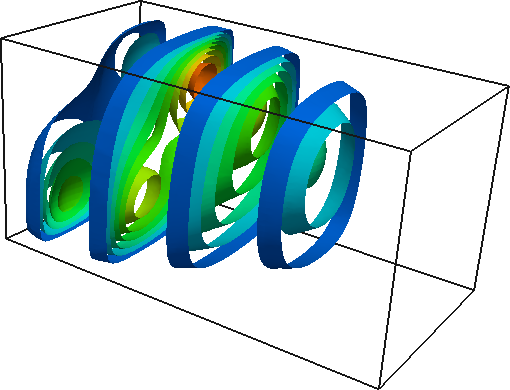
\includegraphics[scale=0.4]{Foto2D+/FEMPretty}}

\subfigure[HiMod]
{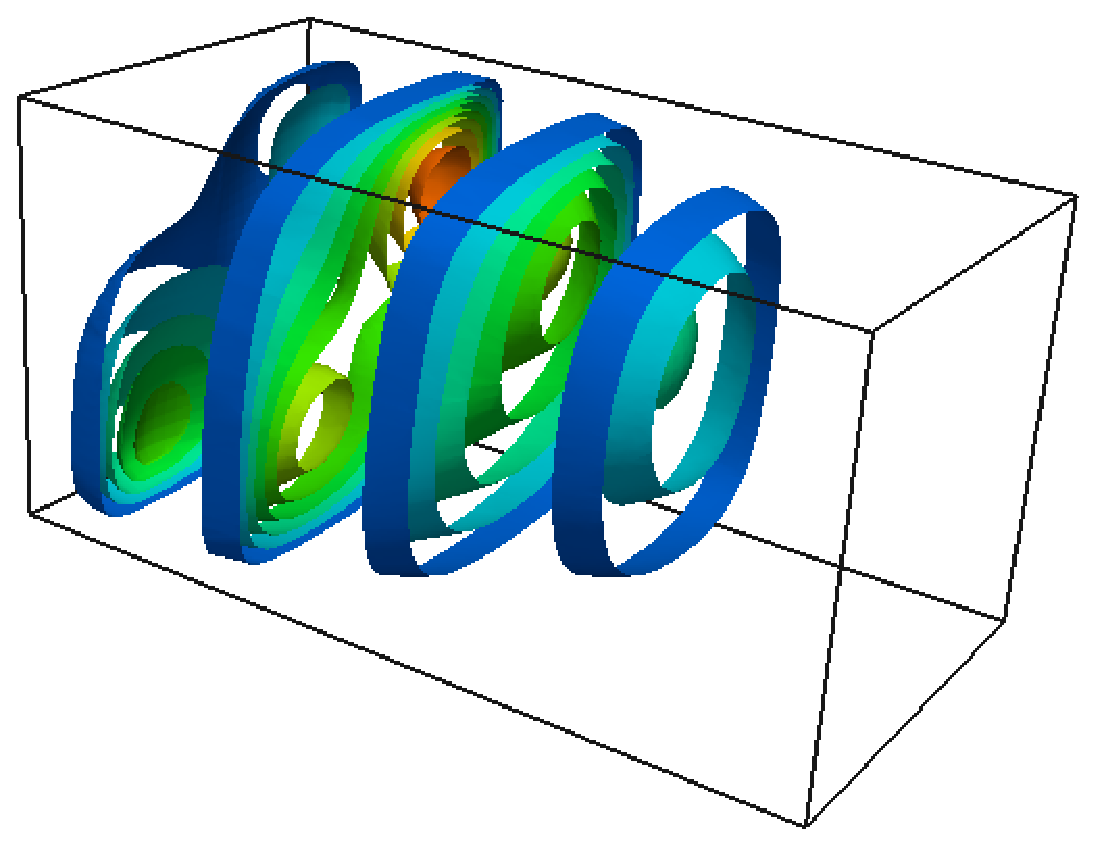
\includegraphics[scale=0.4]{Foto2D+/HiModPretty50}}
\caption{Soluzione FEM a confronto con soluzione HiMod, m=50}
\label{fig:confrontocamini}
\end{figure}
\begin{figure}[!htbp]
\centering
\subfigure[HiMod, m=9]
{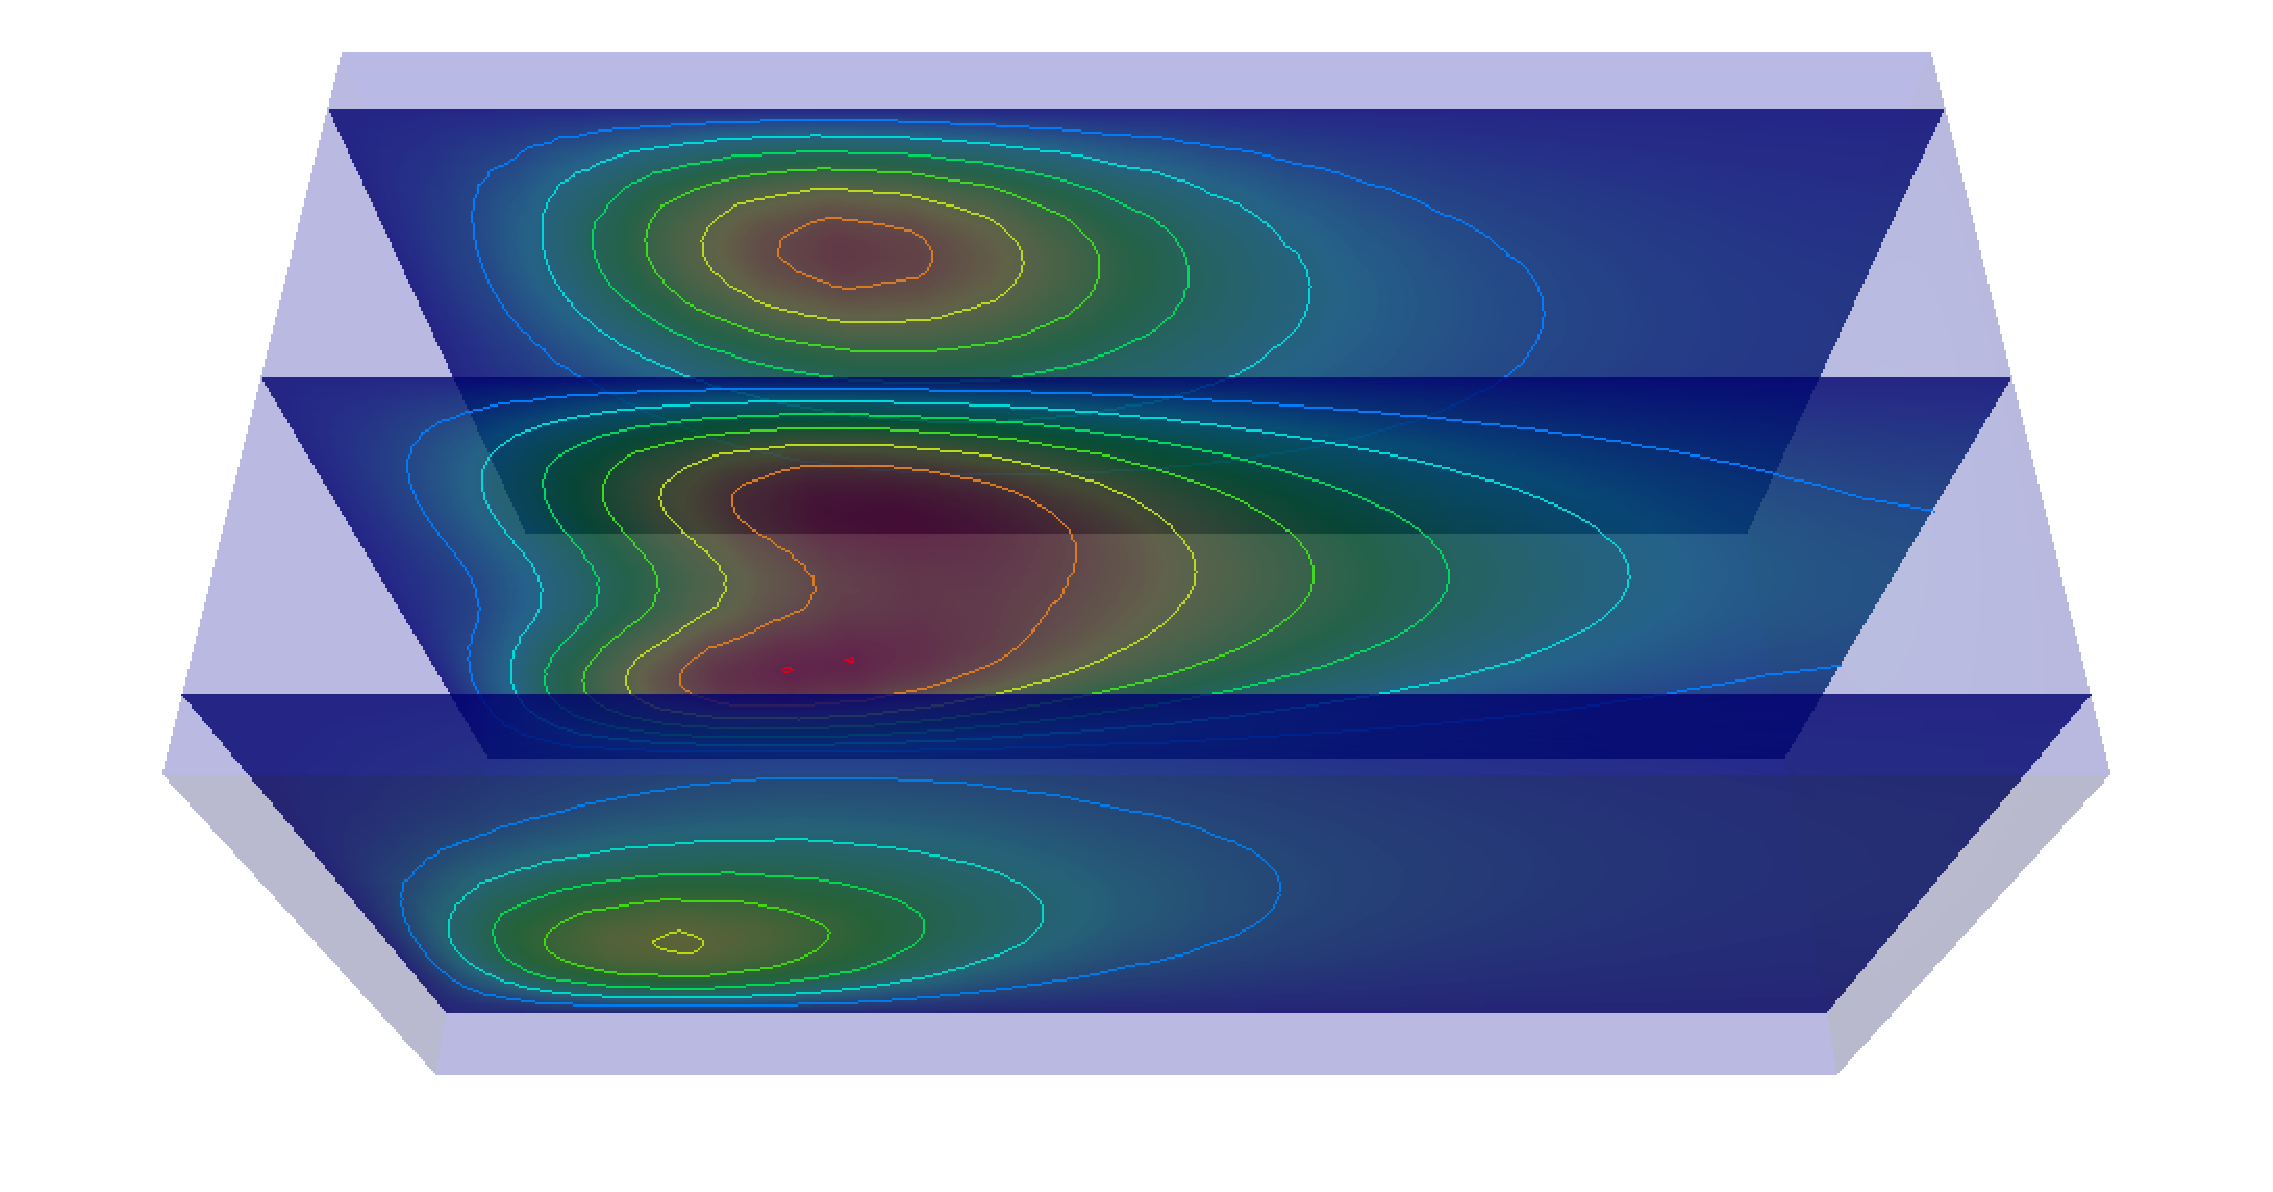
\includegraphics[scale=0.25]{Foto2D+/HiMod_m=9}}

\subfigure[HiMod, m=16]
{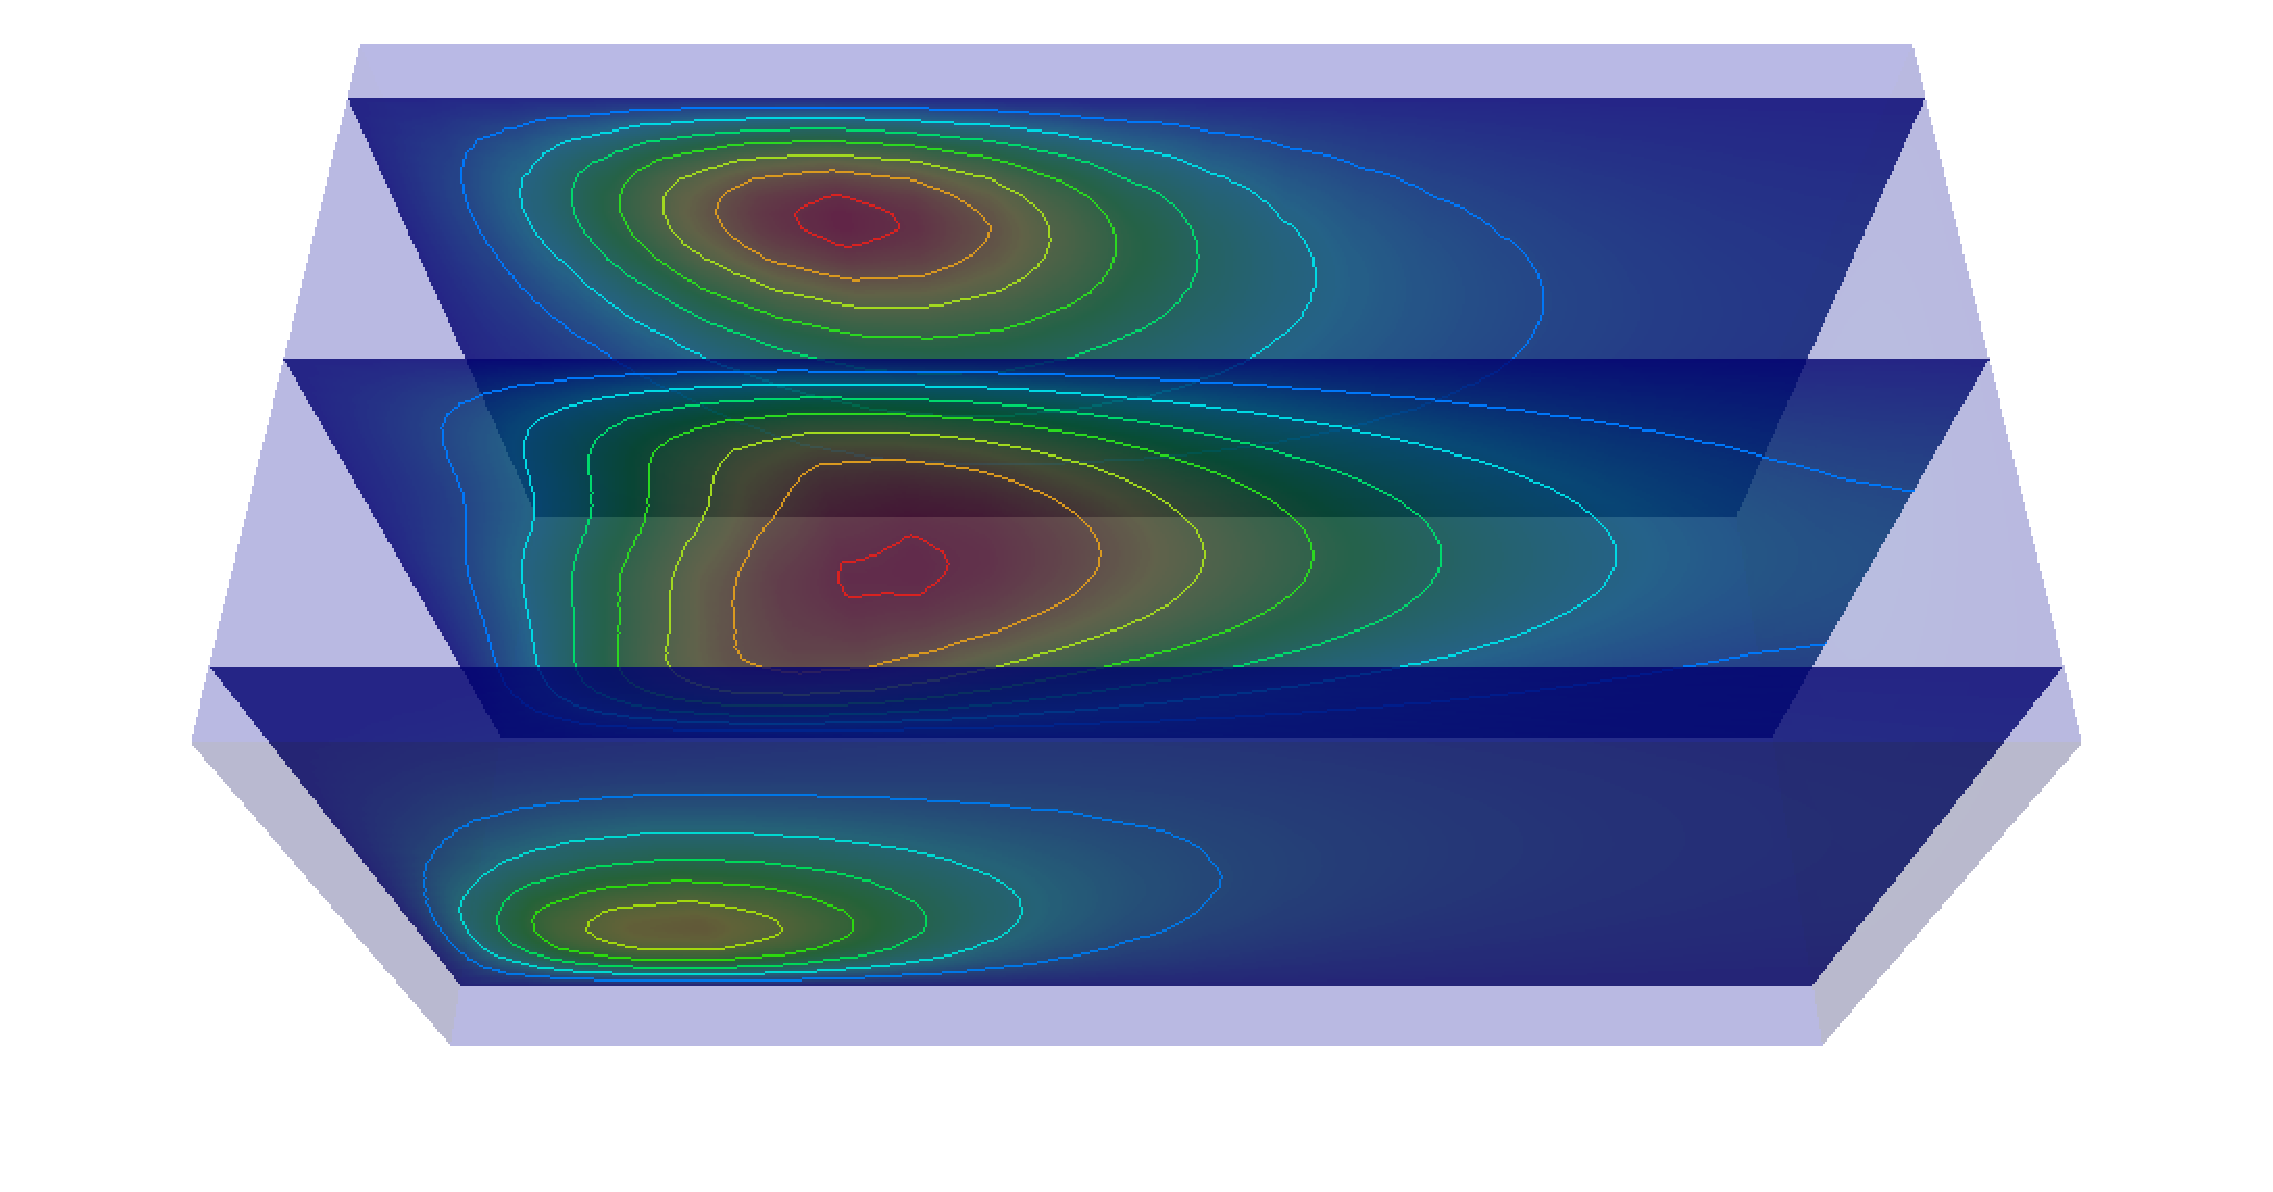
\includegraphics[scale=0.25]{Foto2D+/HiMod_m=16}}

\subfigure[HiMod, m=25]
{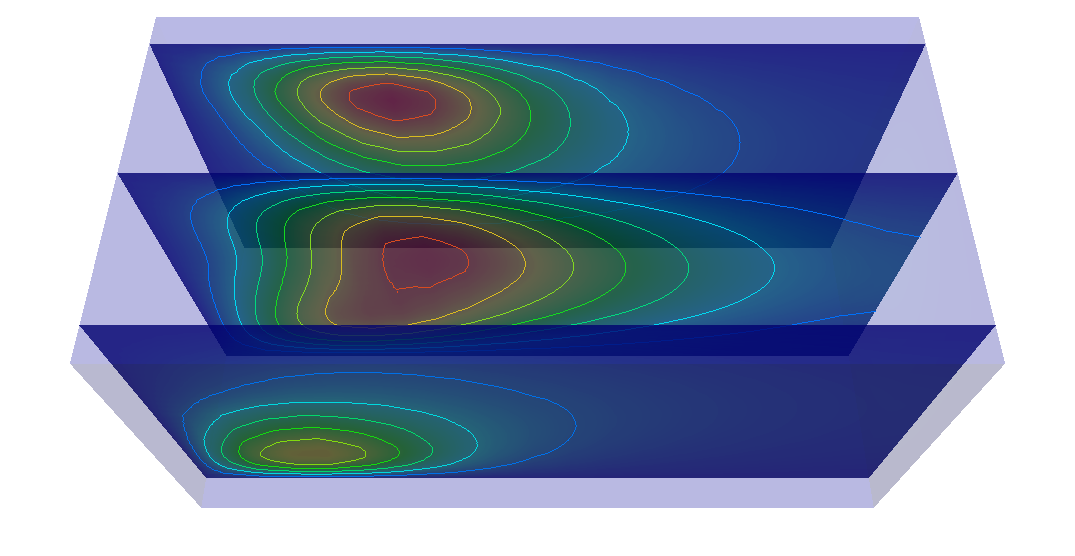
\includegraphics[scale=0.25]{Foto2D+/HiMod_m=25}}

\subfigure[FEM]
{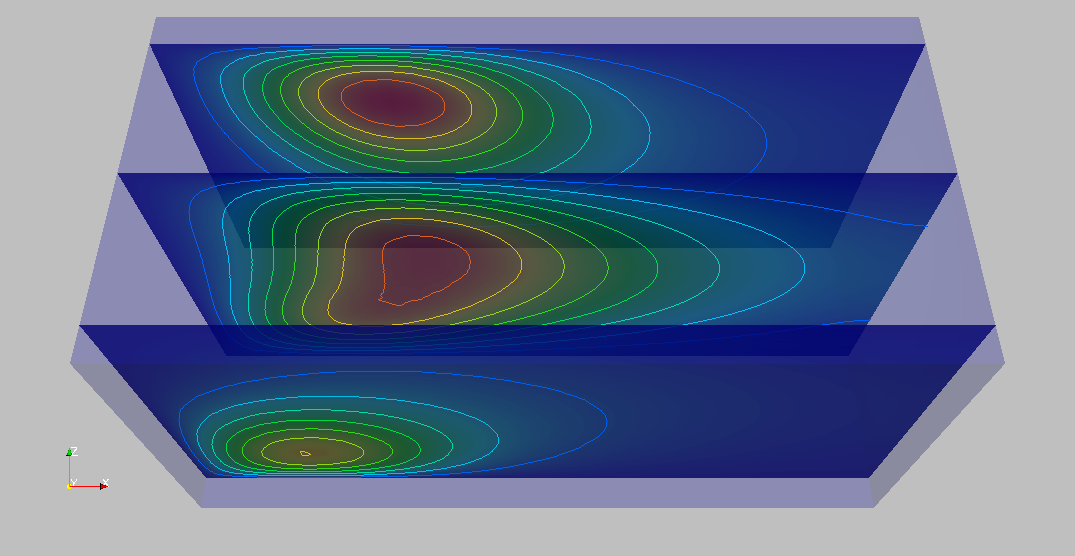
\includegraphics[scale=0.25]{Foto2D+/FEMsolution35}}
\caption{Soluzione FEM a confronto con diversi valori di m}
\label{fig:camini2d+}
\end{figure}
Vediamo che gi\`a con 9 modi \begin{wrapfloat}{figure}{r}{0pt}
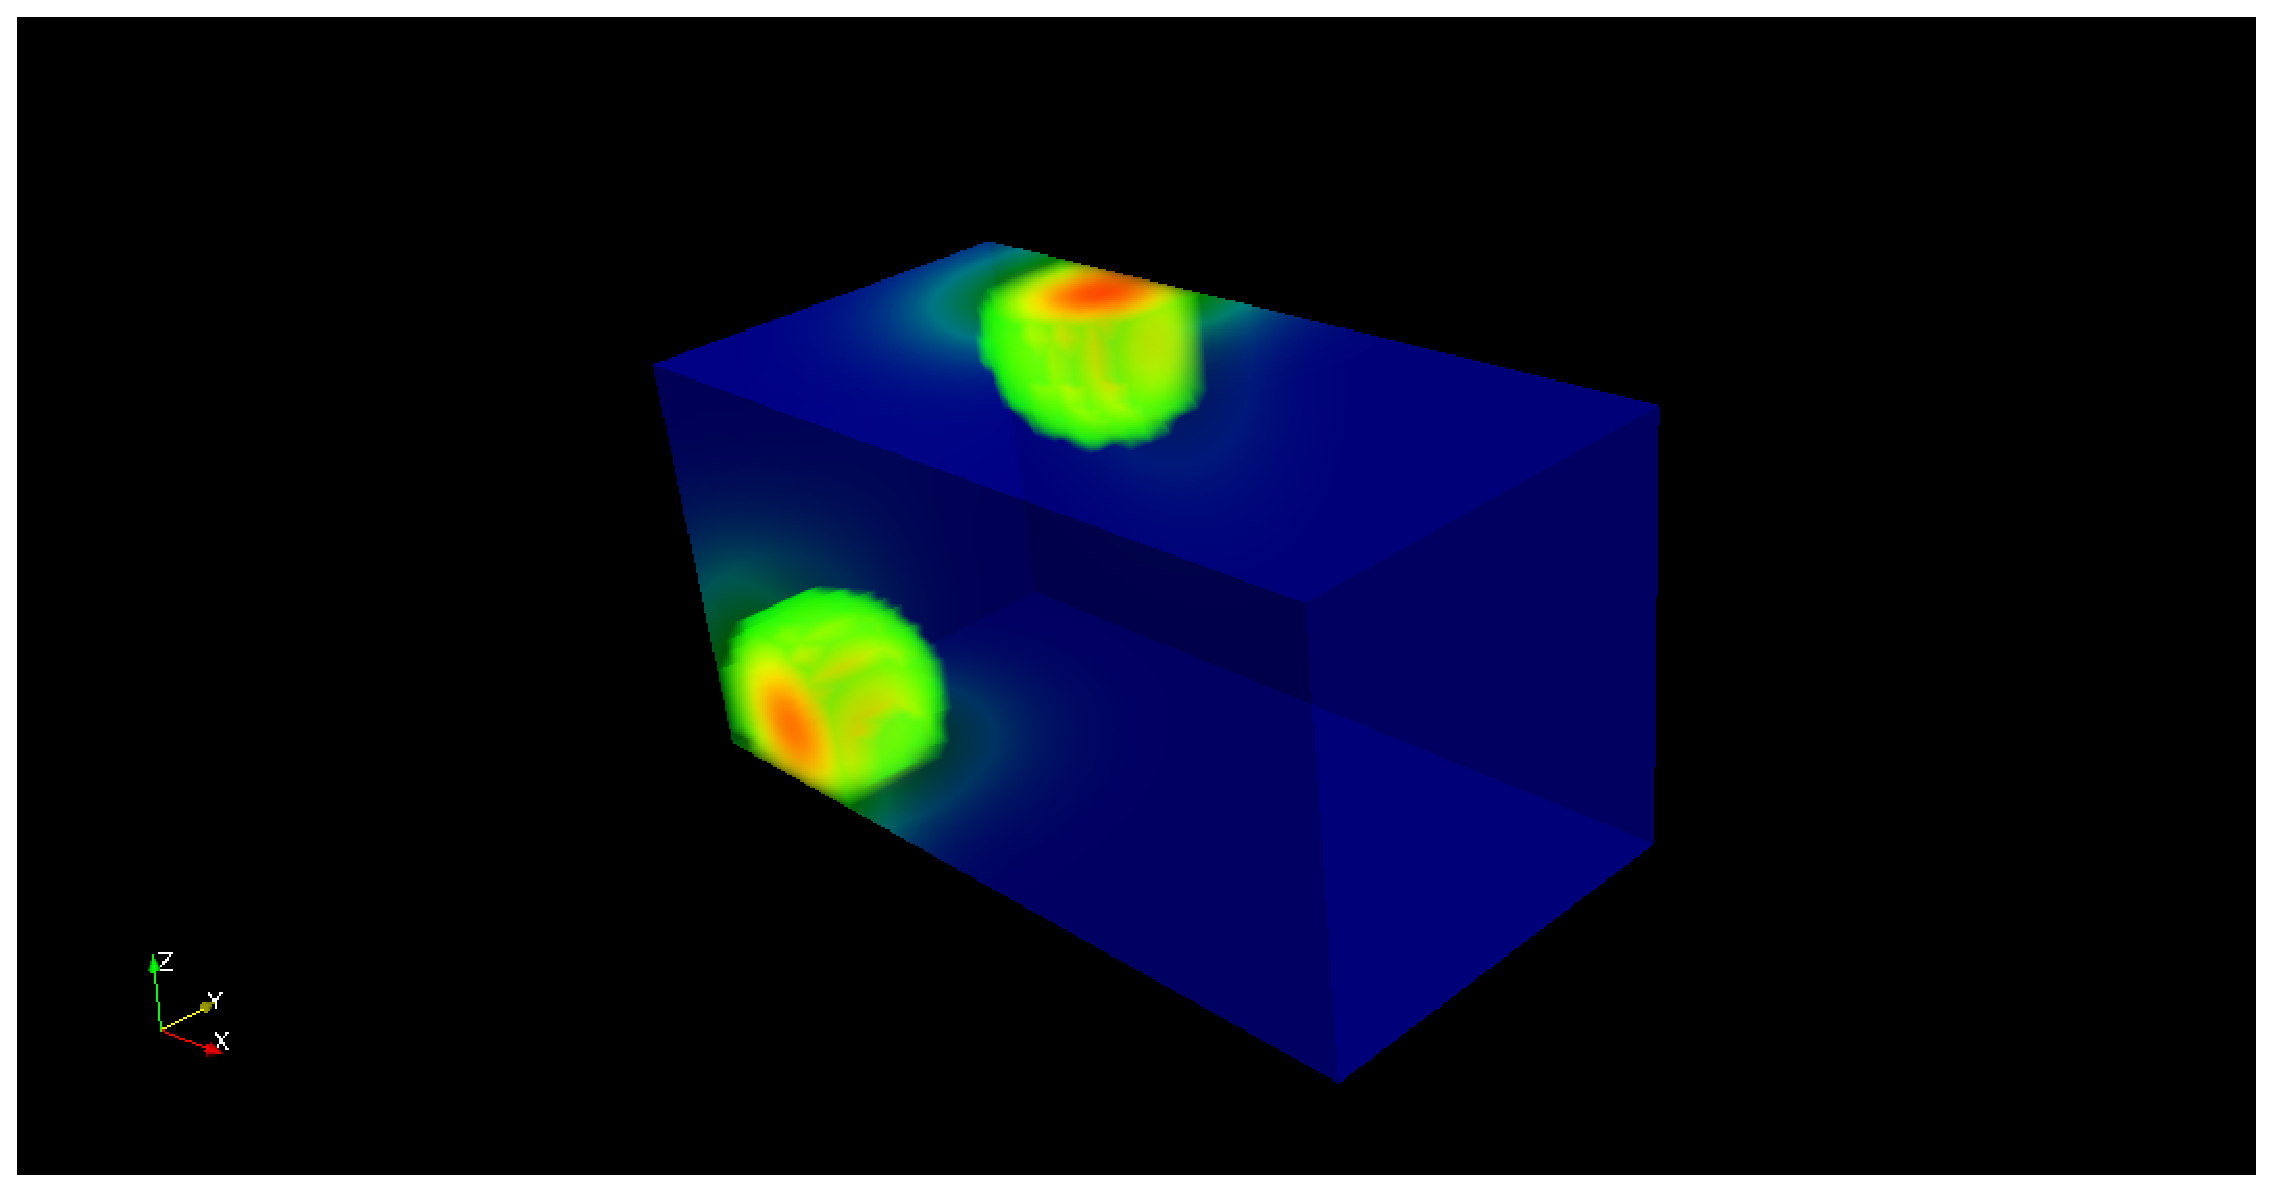
\includegraphics[scale=0.3]{DDDD_ADR/Forceterm}
 \caption{Forzante}
 \label{fig:fcamini}
\end{wrapfloat}la soluzione \`e ragionevole anche se non \`e in grado di cogliere 
bene tutte le caratteristiche della soluzione, con 16 modi ci sono evidenti miglioramenti e con 25 siamo gi\`a a convergenza dal punto di 
vista qualitativo, non abbiamo quindi riportato risultati con pi\`u di 25 modi.
Infine, in figura \ref{fig:camini2D}, riportiamo un'altra visualizzazione della sezione centrale con $y=0.5$.
Anche qui possiamo apprezzare la convergenza.
\begin{figure}[!htbp]
\centering
\subfigure[HiMod, m=9]
{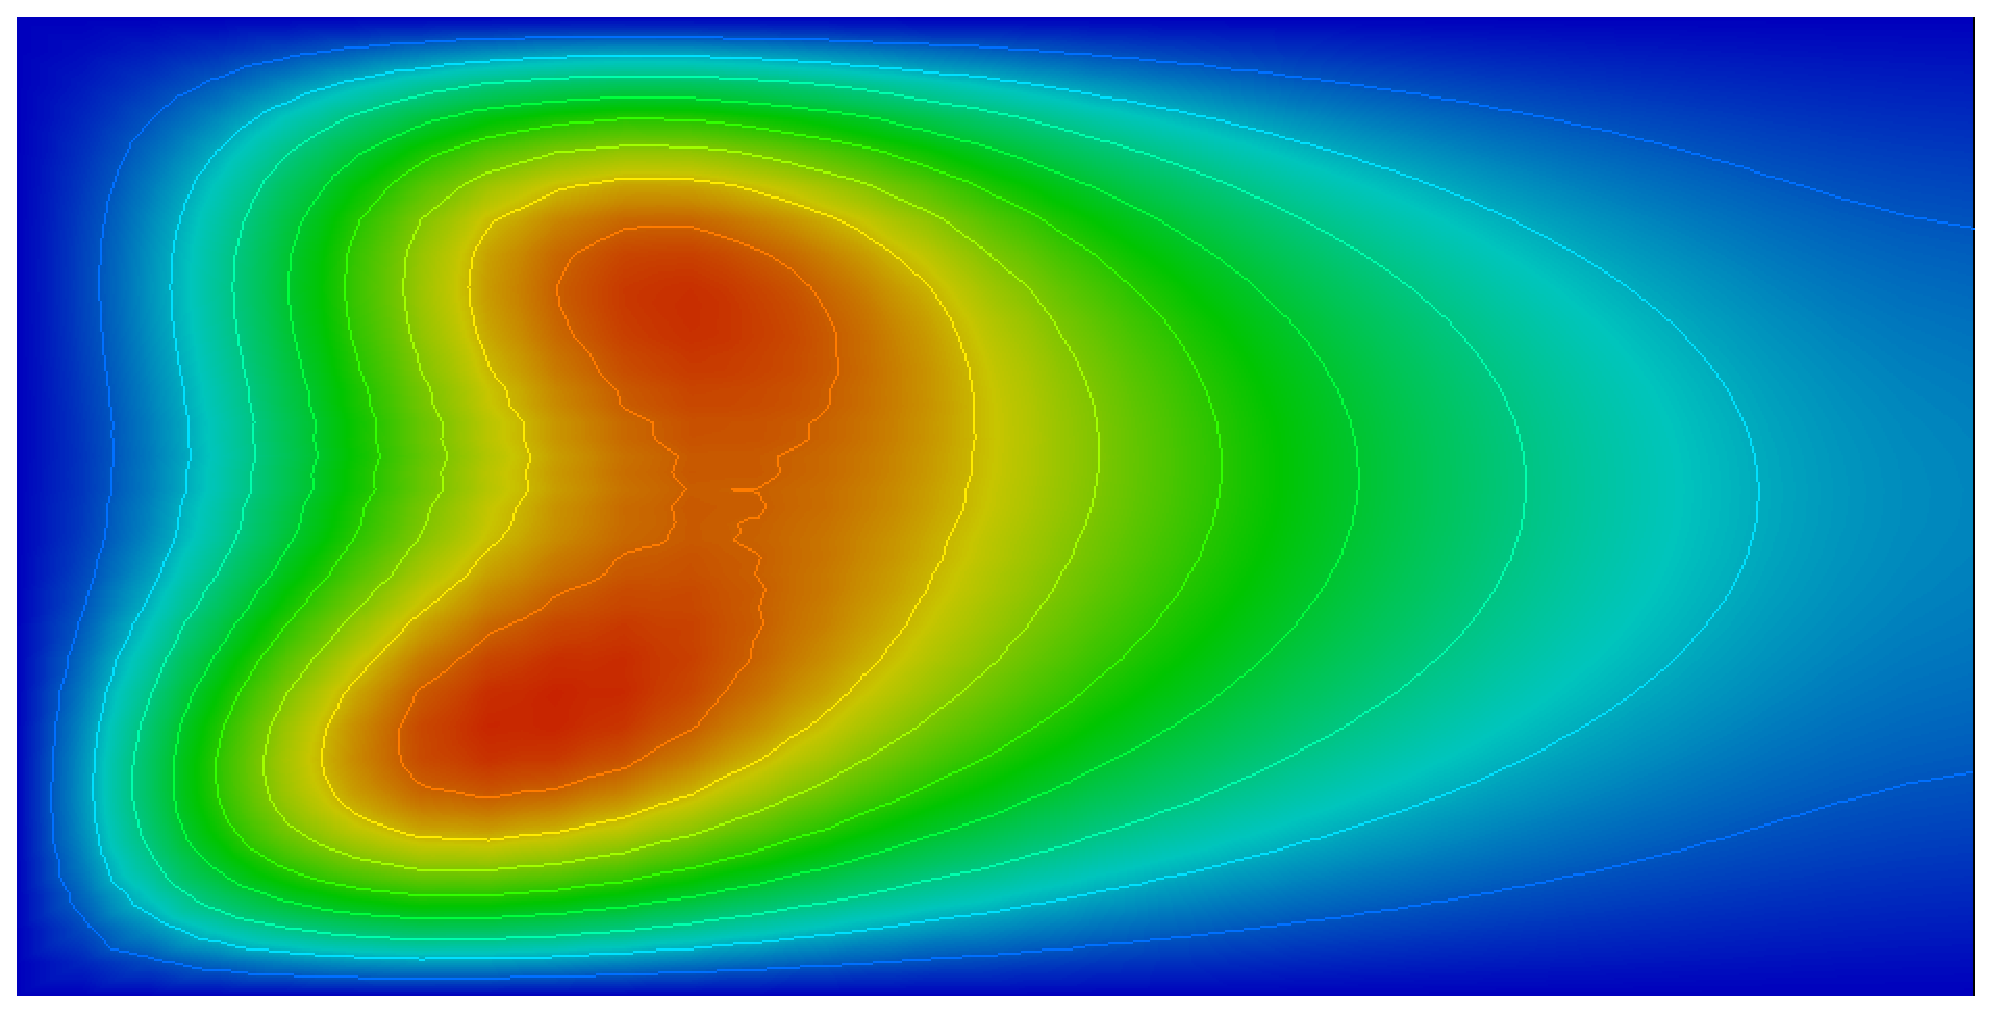
\includegraphics[scale=0.23]{DDDD_ADR/HiMod9slice}}

\subfigure[HiMod, m=16]
{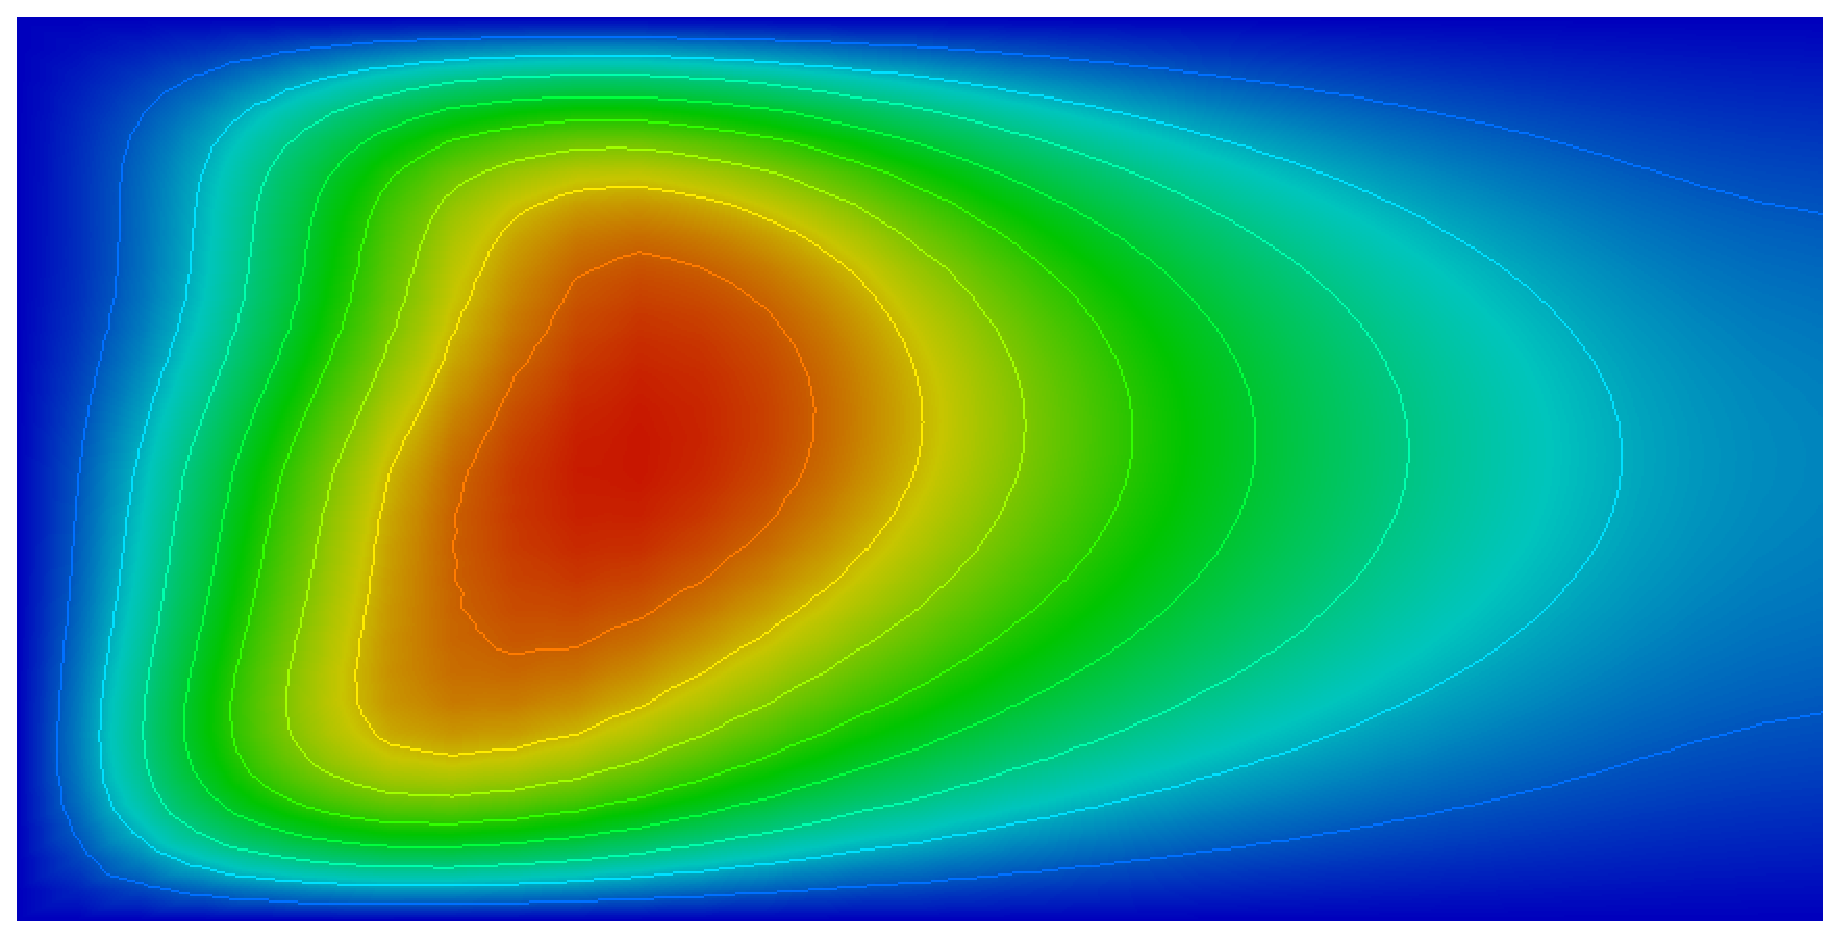
\includegraphics[scale=0.23]{DDDD_ADR/HiMod16slice}}

\subfigure[HiMod, m=25]
{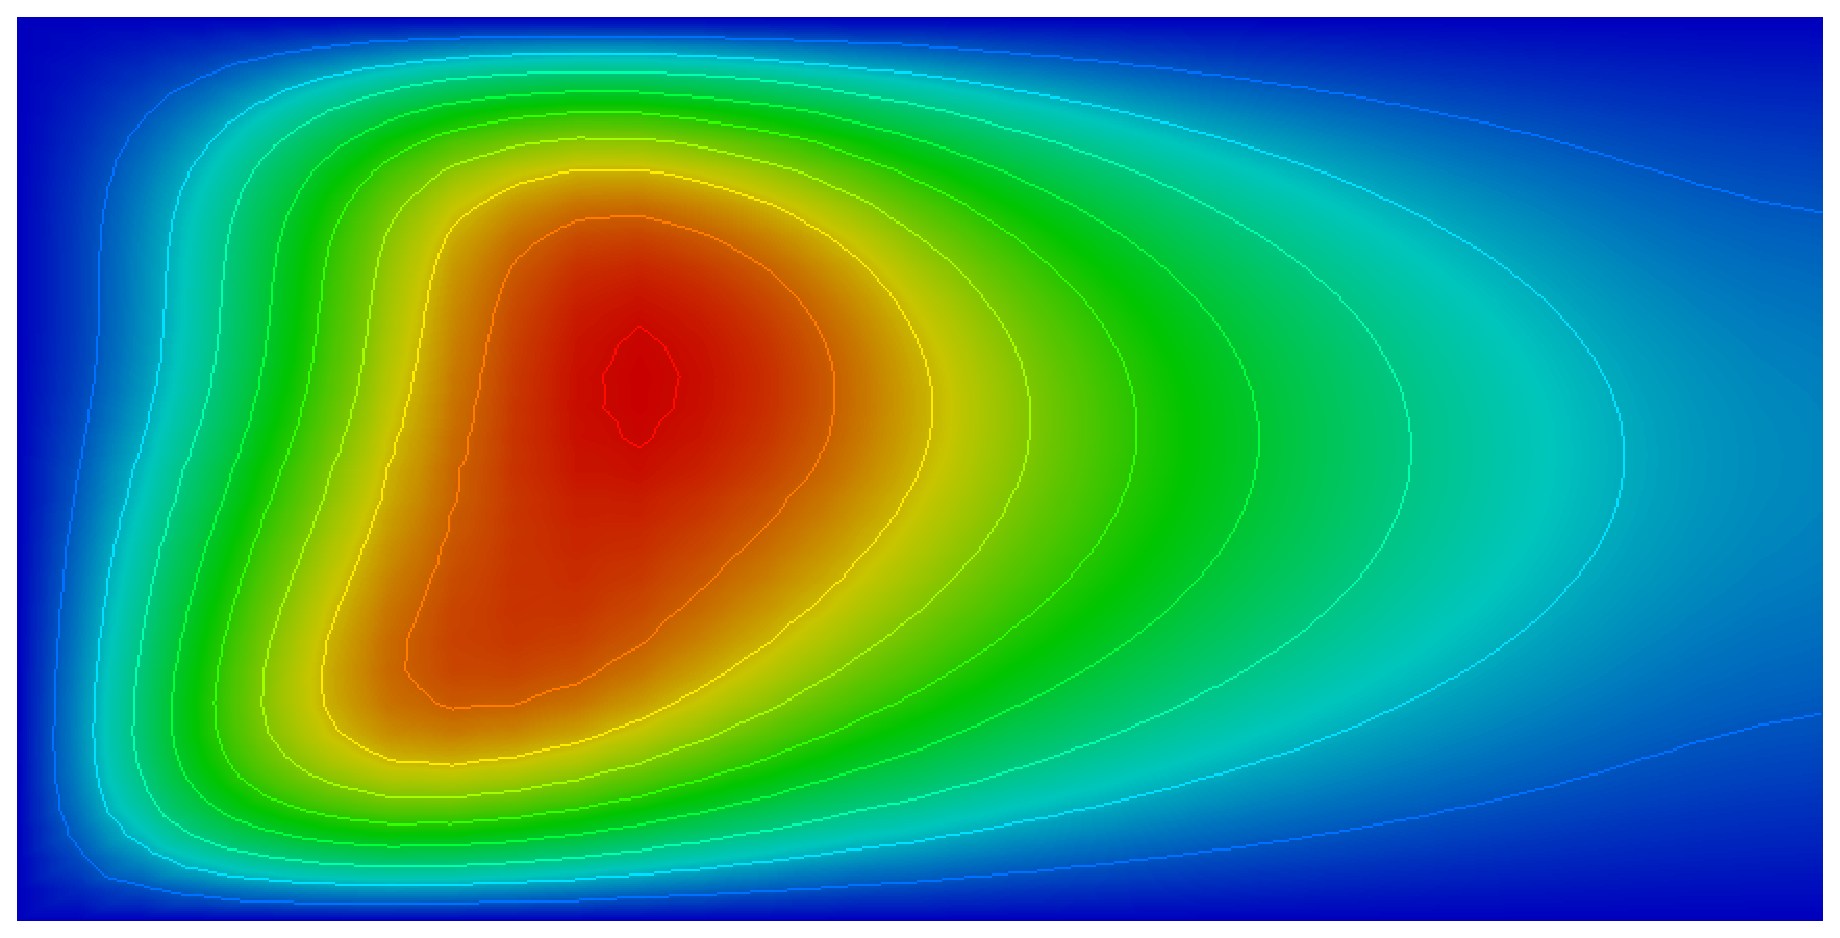
\includegraphics[scale=0.23]{DDDD_ADR/HiMod25slice}}

\subfigure[FEM]
{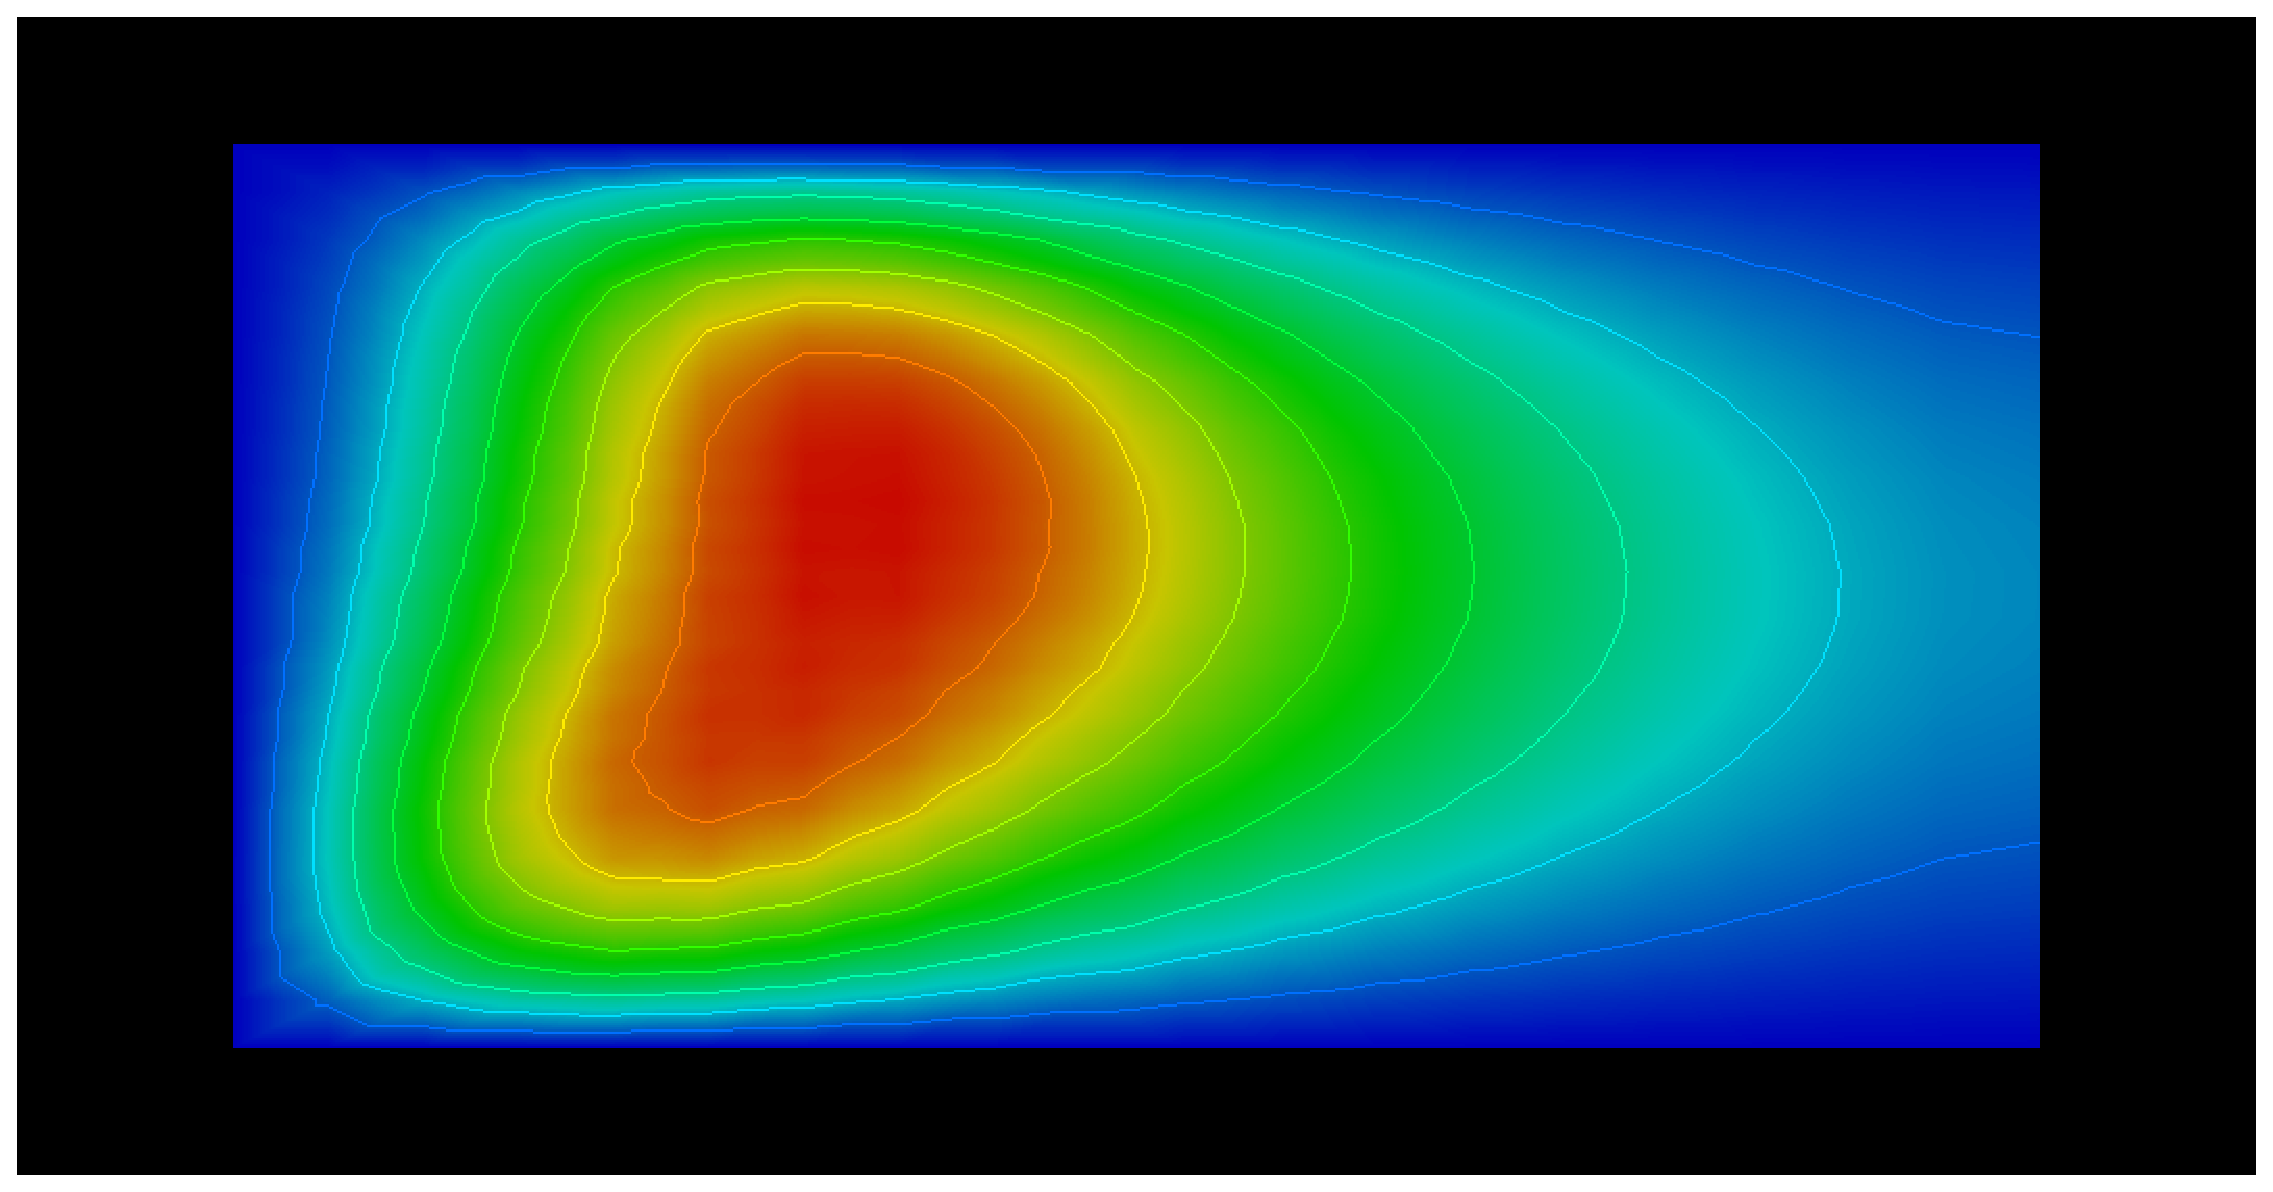
\includegraphics[scale=0.23]{DDDD_ADR/FEMslice}}
\caption{Soluzione FEM a confronto con diversi valori di m}
\label{fig:camini2D}
\end{figure}
Nei successivi esperimenti abbiamo testato diverse combinazioni di dati al bordo e abbiamo cercato di verificare la convergenza del 
metodo. 
\clearpage
\subsection*{Convergenza}
Dal punto di vista teorico la teoria della convergenza per le basi istruite \`e ancora in fase di sviluppo.
Nel caso 2D si ha una convergenza del secondo ordine in $L^2(\Omega)$ rispetto al numero di modi.
In particolare nel caso Dirichlet in 2D usando i P1 in direzione $x$ si ha per $u\in H^2(\Omega)$
\begin{equation}
 \label{eq:stimainl2}
 ||u-u_{m,h}||_{L^2(\Omega)}\leq C ( h^2+m^{-2}) ||u||_{H^2},
\end{equation}
per maggiori dettagli su questo caso si possono trovare in \cite{zilio:himod} teoremi 3.15 e 3.16.

In 3D tenendo conto che $m\sim m_y\cdot m_x$ e con altre considerazioni basate sulle propriet\`a del problema agli autovalori
\`e ragionevole aspettarsi un ordine uno in $L^2(\Omega)$ rispetto al numero di modi, ma la dimostrazione 
non \`e stata ancora terminata.

\begin{figure}[!h]
\centering
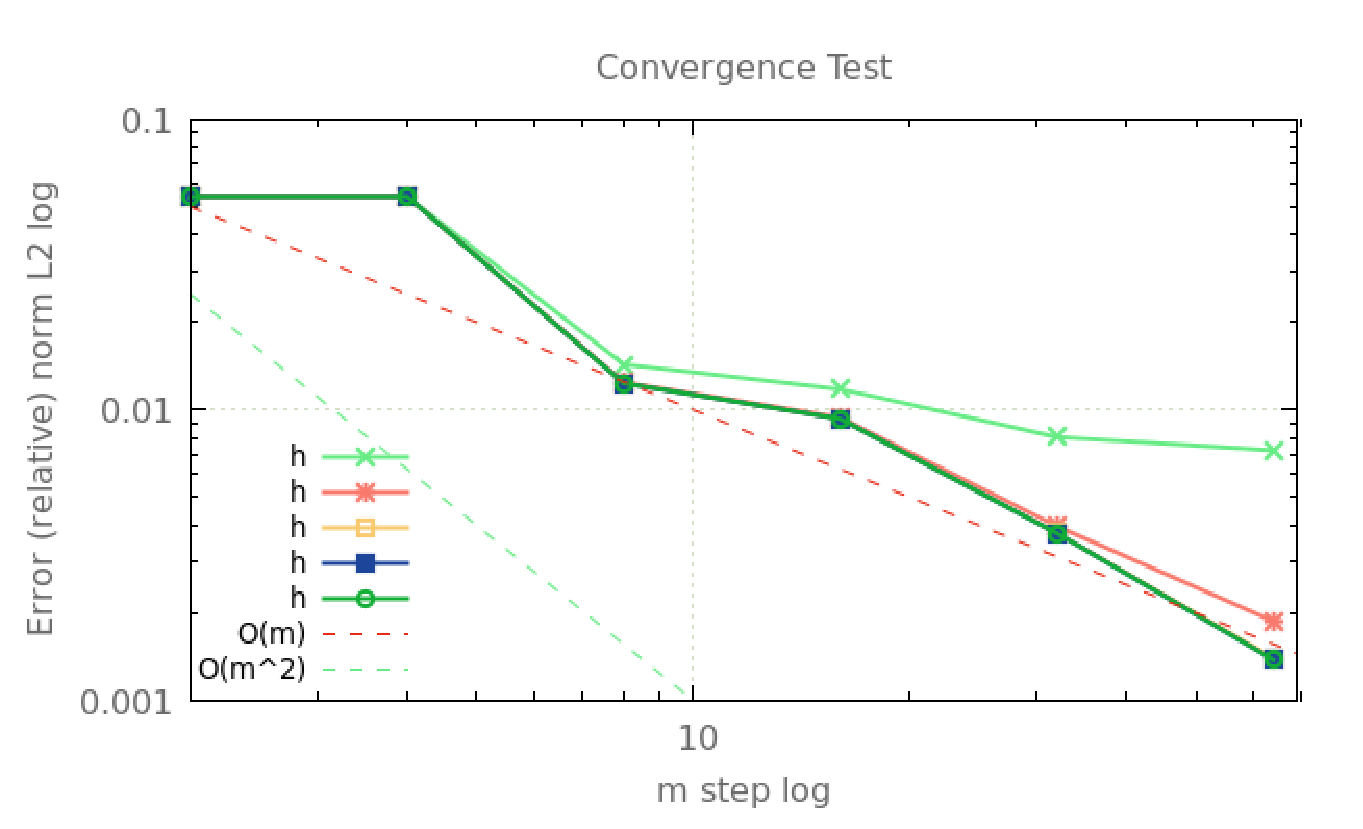
\includegraphics[scale=0.5]{Convergenze/DDDD_ADR}
\caption{Convergenza caso condizioni di Dirichlet}
\label{fig:ddddconv}
\end{figure}

Nella figura \ref{fig:ddddconv} possiamo vedere un caso test con condizioni di Dirichlet sul bordo laterale. Vediamo 
come l'ordine di convergenza sia pari a uno. Vediamo anche che se si usa una griglia elementi finiti troppo 
lasca ad un certo punto l'errore non decresce pi\`u al crescere del numero di modi, perch\`e 
l'errore elementi finiti \`e superiore a quello di modello dovuto all'approssimazione modale.
Vediamo per\`o che riducendo il passo della griglia le curve dell'errore si attestano tutte sulla stessa linea.

\begin{figure}[!h]
\centering
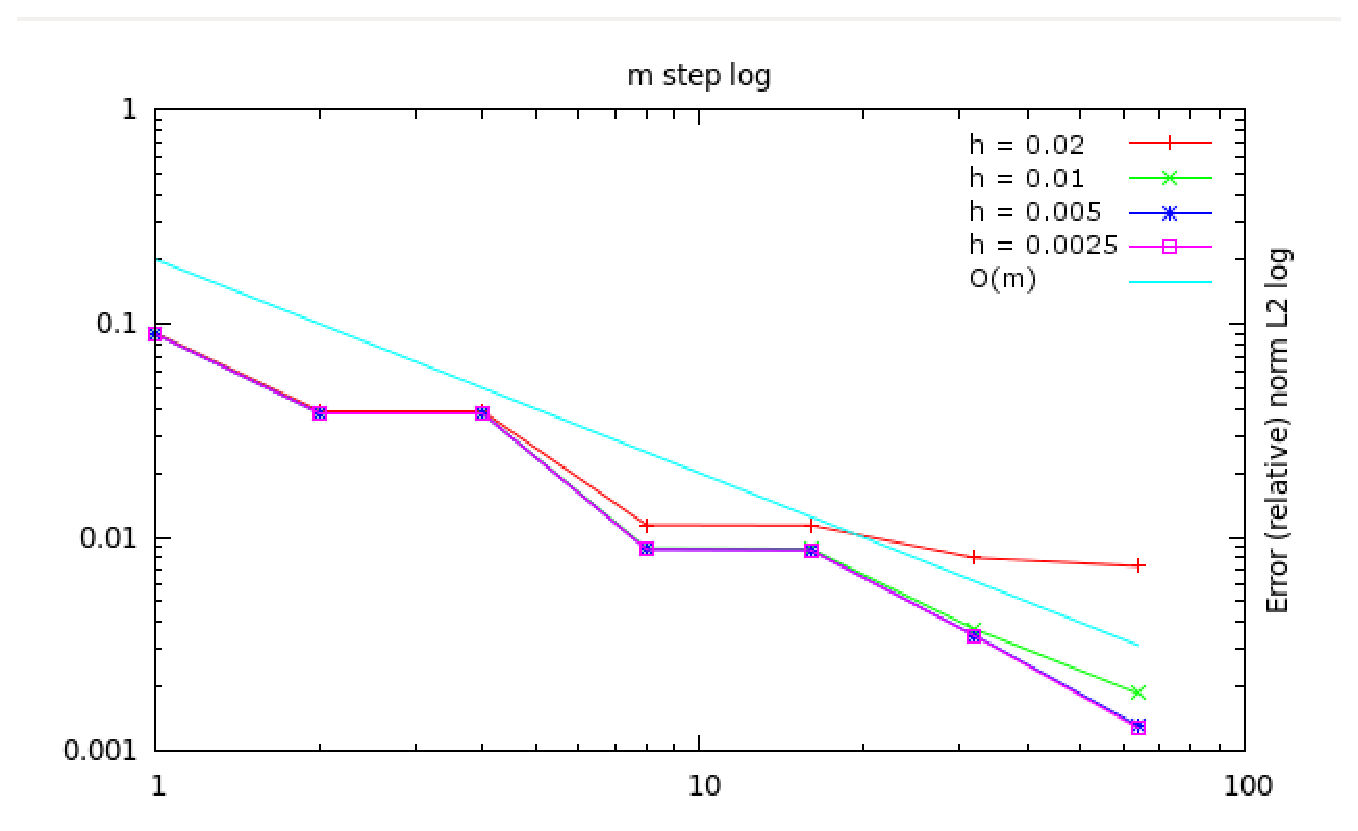
\includegraphics[scale=0.5]{Convergenze/DRDR}
\caption{Convergenza caso condizioni di Dirichlet e di Robin}
\label{fig:drdrconv}
\end{figure}

Nel caso riportato in figura \ref{fig:drdrconv} abbiamo un caso test con condizioni miste sui lati del quadrato:
i lati in basso e in alto hanno condizioni di Dirichlet, mentre i lati a destra e a sinistra hanno condizioni di Robin.
Anche qui possiamo vedere come il grafico di convergenza confermi i risultati attesi dalla teoria.
Infine abbiamo costruito un caso test con condizioni di Robin su tutti i lati. 

\begin{figure}[!h]
\centering
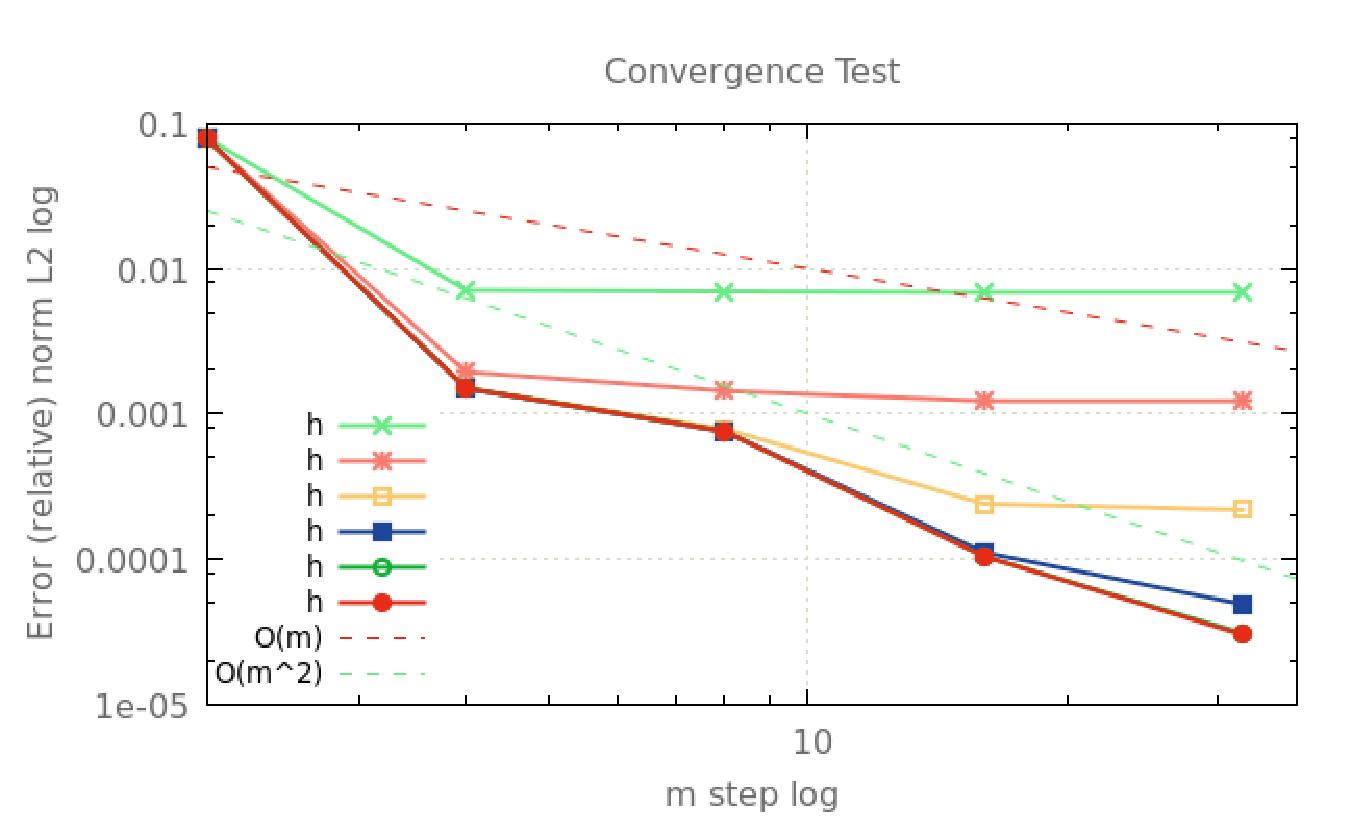
\includegraphics[scale=0.5]{Convergenze/RRRR}
\caption{Convergenza caso condizioni di Robin}
\label{fig:rrrr_conv}
\end{figure}

In figura \ref{fig:rrrr_conv} possiamo 
vedere come l'ordine di convergenza sembra essere superiore alla velocit\`a attesa, questo comportamento in realt\`a 
si verifica anche nei casi test bidimensionali con condizioni al bordo di Robin, dal punto di vista teorico ancora non ci sono 
spiegazioni convincenti, tuttavia questo comportamento si verifica puntualmente.

\begin{figure}[!b]
\centering
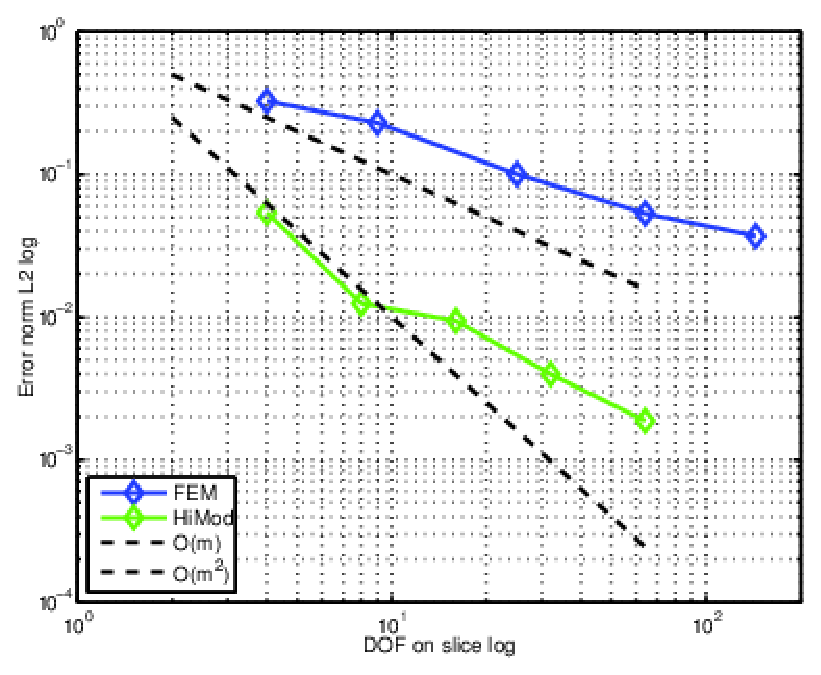
\includegraphics[scale=0.5]{Convergenze/CfrDOF}
\caption{Confronti gradi di libert\`a sulla slice trasversale}
\label{fig:dof}
\end{figure}

Presentiamo inoltre alcuni test per cercare di confrontare gli elementi finiti con HiMod.
In figura \ref{fig:dof} riportiamo sulle ascisse il numero di gradi di libert\`a utilizzati sulla slice trasversale nel caso test con condizioni di Dirichlet e sulle ordinate l'errore in norma $L^2$.
Per gli elementi finiti abbiamo utilizzato una griglia strutturata ed entrambi i metodi condividono la stessa griglia 
in direzione $x$.

\begin{figure}[!b]
\centering
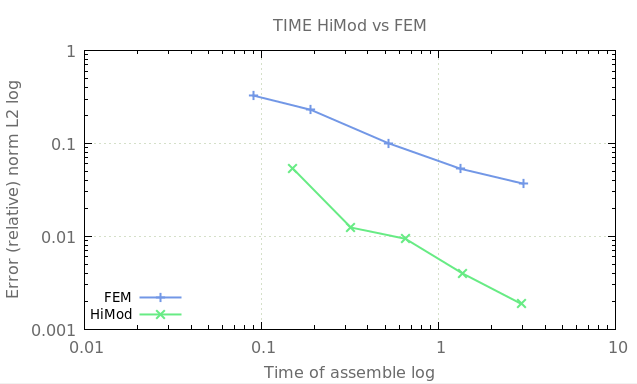
\includegraphics[scale=0.5]{Convergenze/Confronto_tempi}
\caption{Confonto tempi di assemblaggio}
\label{fig:time}
\end{figure}

Si vede come a parit\`a di precisione, con himod sia possibile utilizzare meno gradi di libert\`a in direzione trasversale.
Tuttavia questo dipende anche dal caso test, perch\`e l'ordine di convergenza \`e lo stesso, quindi tutto dipende dalla 
costante davanti alla stima dell'errore. \`E chiaro che se la soluzione non presenta dinamiche particolarmente complesse in direzione trasversale,
se la base scelta \`e buona gi\`a con i primi modi si potranno cogliere le caratteristiche principali e dunque la curva HiMod
in figura \ref{fig:dof} si trover\`a al di sotto della curva per gli elementi finiti.

Infine, sempre sul caso test con condizioni di Dirichlet, abbiamo cercato di capire quanto tempo impiega l'assemblaggio della matrice
rispetto all'analogo test assemblato con \texttt{ADRAssembler} di \texttt{LifeV}.
I risultati si possono vedere in figura \ref{fig:time} e vediamo come, a parit\`a di precisione, il tempo di assemblaggio 
della matrice sia minore che nel caso elementi finiti, ci\`o \`e dovuto al minor numero di gradi di libert\`a.

\clearpage
\nocite{*}%esempio di prova
\addcontentsline{toc}{chapter}{Bibliografia}
\bibliographystyle{alpha}
\bibliography{pacs}

\end{document}